\documentclass[english,sectioncirclenumberstyle]{ciadbeamer}

\usepackage{lipsum}

\usepackage[utf8]{inputenc}
\usepackage{algpseudocode}
\usepackage{multicol}

\graphicspath{{./docfigs/}}

\title{Documentation of the CIAD Theme for Beamer}
\subtitle{Version \insertciadbeamerthemeversion}

\author[S.~Galland]{St\'ephane~Galland}

\keywords{Beamer; Theme; CIAD; UTBM; UBE; Documentation}
\subject{Beamer Theme for CIAD Laboratory}

\finalslidetext{End of the Documentation}

\usefootlinewithsections

\pgfdeclareimage[height=.2cm]{fakeutbmlogoinpartners}{utbmgraylogo}
\pgfdeclareimage[height=.2cm]{fakeubelogoinpartners}{ubegraylogo}
\pgfdeclareimage[height=.2cm]{fakecarnotlogoinpartners}{carnotgraylogo}
\pgfdeclareimage[height=.25cm]{fakeciadlogointitle}{ciadlogointitle}
\pgfdeclareimage[height=.25cm]{fakeutbmlogointitle}{utbmlogointitle}
\pgfdeclareimage[height=.25cm]{fakeubelogointitle}{ubelogointitle}
\pgfdeclareimage[height=.25cm]{fakeuserlogointitle}{utbmlogo}

\makeatletter
\let\fakebackground\beamer@theme@ciad@outer@background
\makeatother

\makeatletter
\let\fakeoldunderline\beamer@theme@ciad@oldunderline
\makeatother

\newcommand{\fakeslide}[3][fakeciadlogointitle]{
	\framebox{\begin{minipage}{.4\paperwidth}
		\begin{picture}(0,90)
			\put(-3,86){\scalebox{0.414}{\fakebackground}}
			\put(1,88){\textcolor{frametitle.fg}{\tiny #2}}
			\ifthenelse{\equal{a#1}{a}}{}{\put(165,86){\pgfuseimage{#1}}}
			#3
			\put(120,-1){\pgfuseimage{fakeutbmlogoinpartners}\hspace{0.05cm}\hspace{0.05cm}\pgfuseimage{fakeubelogoinpartners}\hspace{0.05cm}\pgfuseimage{fakecarnotlogoinpartners}}
		\end{picture}
	\end{minipage}}
}

\begin{document}

%%%%%%%%%%%%%%%%%%%%%%%%%%%%%%%%%%%%%%%%%%%%%%%%
\begin{frame}{Introduction}
	\begin{itemize}
	\item This document explains the {\LaTeX} macros that are provided by the CIAD theme for beamer.
	\vfill
	\item To use the CIAD theme for beamer, you must:
		\begin{enumerate}
		\item Install the files of the CIAD theme inside your {\LaTeX} distribution.
		\item Create a document, which uses the document class: \texttt{ciadbeamer}
		\end{enumerate}
	\end{itemize}
\end{frame}

\begin{frame}{Major Features}
	\begin{itemize}
	\item Provide a presentation style related to the research group of the CIAD laboratory located at the UTBM and UBE.
	\vfill
	\item Add a title slide (with label \texttt{titleslide} for \texttt{{\textbackslash}hyperlink}) as the first slide.
	\vfill
	\item Add a final slide at the end of the presentation to avoid ``black'' screen at the end of the presentation.
	\vfill
	\item Provide high level macros for building the slides.
	\end{itemize}
\end{frame}

\begin{frame}{Read the Beamer Documentation}
	\huge
	\alertbox{It is recommended to read the user guide of Beamer for obtain a view of the available macros.}
	\vspace{2em}
	\alertbox*{\url{http://texdoc.net/texmf-dist/doc/latex/beamer/doc/beameruserguide.pdf}}
\end{frame}

%%%%%%%%%%%%%%%%%%%%%%%%%%%%%%%%%%%%%%%%%%%%%%%%%%
\tableofcontentslide

%%%%%%%%%%%%%%%%%%%%%%%%%%%%%%%%%%%%%%%%%%%%%%%%%%
\section{Predefined Values}
\sectionsintoc{1-7}
\sectiontableofcontentslide

\subsection{Colors}

\begin{frame}{{\LaTeX}\ Colors}
	\begin{itemize}
	\item The CIAD theme defines the colors for the macros provided by the \texttt{xcolor} package:
		\begin{itemize}
		\item \texttt{CIADblue} : \fbox{\textcolor{CIADblue}{Example}} \colorbox{CIADblue}{\textcolor{white}{Example}}
		\item \texttt{CIADmagenta} : \fbox{\textcolor{CIADmagenta}{Example}} \colorbox{CIADmagenta}{\textcolor{white}{Example}}
		\item \texttt{CIADgreen} : \fbox{\textcolor{CIADgreen}{Example}} \colorbox{CIADgreen}{\textcolor{white}{Example}}
		\item \texttt{CIADdarkgreen} : \fbox{\textcolor{CIADdarkgreen}{Example}} \colorbox{CIADdarkgreen}{\textcolor{white}{Example}}
		\item \texttt{CIADlightgreen} : \fbox{\textcolor{CIADlightgreen}{Example}} \colorbox{CIADlightgreen}{\textcolor{black}{Example}}
		\item \texttt{CIADlightestgreen} : \fbox{\textcolor{CIADlightestgreen}{Example}} \colorbox{CIADlightestgreen}{\textcolor{black}{Example}}
		\item \texttt{CIADdarkmagenta} : \fbox{\textcolor{CIADdarkmagenta}{Example}} \colorbox{CIADdarkmagenta}{\textcolor{white}{Example}}
		\item \texttt{CIADlightmagenta} : \fbox{\textcolor{CIADlightmagenta}{Example}} \colorbox{CIADlightmagenta}{\textcolor{white}{Example}}
		\item \texttt{CIADlightestmagenta} : \fbox{\textcolor{CIADlightestmagenta}{Example}} \colorbox{CIADlightestmagenta}{\textcolor{black}{Example}}
		\end{itemize}
	\end{itemize}
\end{frame}

\begin{frame}{{\LaTeX}\ Colors \insertcontinuationtext}
	\begin{itemize}
	\item The CIAD theme defines the colors for the macros provided by the \texttt{xcolor} package:
		\begin{itemize}
		\item \texttt{CIADdarkgray} : \fbox{\textcolor{CIADdarkgray}{Example}} \colorbox{CIADdarkgray}{\textcolor{white}{Example}}
		\item \texttt{CIADlightgray} : \fbox{\textcolor{CIADlightgray}{Example}} \colorbox{CIADlightgray}{\textcolor{black}{Example}}
		\item \texttt{CIADlightestgray} : \fbox{\textcolor{CIADlightestgray}{Example}} \colorbox{CIADlightestgray}{\textcolor{black}{Example}}
		\end{itemize}
	\end{itemize}
\end{frame}

\begin{frame}{Beamer Colors}
	\begin{itemize}
	\item The CIAD theme defines color for beamer, that may be used with the macro \texttt{{\textbackslash}usebeamercolor\{color\_name\}}:
		\begin{itemize}
		\item \texttt{code keyword} : \fbox{\usebeamercolor[fg]{code keyword}Example}
		\vfill
		\item \texttt{code string} : \fbox{\usebeamercolor[fg]{code string}Example}
		\vfill
		\item \texttt{code comment} : \fbox{\usebeamercolor[fg]{code comment}Example}
		\end{itemize}
	\end{itemize}
\end{frame}

\subsection{Styles}
\begin{frame}{Beamer Templates}
	\begin{itemize}
	\item The CIAD theme defines the specific templates for Beamer. These templates could be used with 
		\texttt{{\textbackslash}usebeamertemplate\{name\}}:
		\begin{itemize}
		\item \texttt{code basic style} : the style for the standard text in a program or an algorithm. 
		\vfill
		\item \texttt{code inline style} : the style for the standard text in a program or an algorithm when it is displayed inline. 
		\vfill
		\item \texttt{code identifier style} : the style for the identifiers in a program or an algorithm. 
		\vfill
		\item \texttt{code keyword style} : the style for the keywords in a program or an algorithm. 
		\end{itemize}
	\end{itemize}
\end{frame}

%%%%%%%%%%%%%%%%%%%%%%%%%%%%%%%%%%%%%%%%%%%%%%%%%%
\section{Class Options and Document Declaration}
\sectionsintoc{1-6}
\sectiontableofcontentslide

\subsection{Class Options}

\begin{frame}[t]{Class Options}
	The document class \texttt{ciadbeamer} supports the following options.
	\begin{block}{Presentation language}
		\begin{itemize}
		\item \texttt{english}: the slides are written in English (this is the default).
		\item \texttt{french}: the slides are written in French.
		\end{itemize}
	\end{block}
	\begin{block}{Automatic slides}
		\begin{itemize}
		\item \texttt{nocover}: do not add a slide for the title and the ``thanks''.
		\item \texttt{thanksslide}: add a slide with the word ``Thanks'' at the end (this is the default). 
		\item \texttt{questionslide}: add a slide with the word ``Question'' at the end. 
		\item \texttt{repeattitleslide}: add the title slide at the end.
		\end{itemize}
	\end{block}
\end{frame}

\begin{frame}[t]{Class Options \insertcontinuationtext}
	\begin{block}{Slide numbering}
		\begin{itemize}
		\item \texttt{textnumberstyle}: the frame numbers are output as text.
		\item \texttt{circlenumberstyle}: the frame numbers are output in a circle.
		\item \texttt{sectioncirclenumberstyle}: the frame numbers are output in a circle.
		\item \texttt{partcirclenumberstyle}: similar to \texttt{circlenumberstyle} except that the indicator is reset at the start of each part.
		\item \texttt{partsectioncirclenumberstyle}: similar to \texttt{sectioncirclenumberstyle} except that the indicator is reset at the start of each part.
		\item \texttt{nonumberstyle}: the frame numbers are not output.
		\end{itemize}
	\end{block}
	\begin{block}{Example}
		\hyperlink{progressbartypes}{\beamergotobutton{See example}}
	\end{block}
\end{frame}

\begin{frame}[t]{Class Options \insertcontinuationtext}
	\begin{block}{Footline and Headline}
		\begin{itemize}
		\item \texttt{lablogo} and \texttt{nolablogo}: enable or disable the logos of the main institutions (lab, universities, etc.) in the foot line.
		\item \texttt{utbmlogo} and \texttt{noutbmlogo}: enable or disable the logo of "Universit\'e de Technologie de Belfort-Montb\'eliard" in the foot line.
		\item \texttt{ubelogo} and \texttt{noubelogo}: enable or disable the logo of "Universit\'e de Bourgogne" in the foot line.
		\item \texttt{carnotlogo} and \texttt{nocarnotlogo}: enable or disable the logo of "Institut Carnot" in the foot line.
		\item \texttt{frenchrepublic} and \texttt{nofrenchrepublic}: enable or disable the logo of the French Republic in the head line.
		\end{itemize}
	\end{block}
\end{frame}

\begin{frame}[t]{Class Options \insertcontinuationtext}
	\begin{block}{Hyphenation}
		\begin{itemize}
		\item \texttt{hyphenation} and \texttt{nohyphenation}: enable or disable the hyphenation of the text on the slides.
		\end{itemize}
	\end{block}
	\begin{block}{Handout --- Free space beside slides for hand notes}
		\begin{itemize}
		\item \texttt{handout} and \texttt{nohandout}: enable or disable the generation of the handout document.
		\end{itemize}
	\end{block}
\end{frame}

\begin{frame}[t]{Class Options \insertcontinuationtext}
	\begin{block}{Fancy Title Page}
		\begin{itemize}
		\item \texttt{titlefancyletters} and \texttt{notitlefancyletters}: enable or disable the fancy rendering of the first letters of the words with a specific color into the title frame.
		\item \texttt{allfancyletters}: If the previous option is true, all the letters are colored. Otherwise only the upper case letters are colored.
		\item \texttt{fancyframetitle} and \texttt{nofancyframetitle}: enable or disable the rendering of the first group of words and the second group in the frame's title.
		\end{itemize}
	\end{block}
\end{frame}

\begin{frame}{Class Options \insertcontinuationtext}
	\alertbox{All the options accepted by Beamer are also accepted.}
\end{frame}

\subsection{Title, Subtitle and Front Page}

\begin{frame}{Title and Subtitle}
	\begin{block}{Title}
		Use the macro: \texttt{{\textbackslash}title\{title of the document\}}
	\end{block}
	\vfill
	\begin{block}{Subtitle}
		Use the macro: \texttt{{\textbackslash}subtitle\{subtitle of the document\}}
	\end{block}
	\vfill
	\alertbox{These macros must be put in the preamble of your document.}
\end{frame}

\begin{frame}[t]{{Change the Figures} on the Title Slide}
	The title page contains a background divided into several parts:
	\begin{center}
		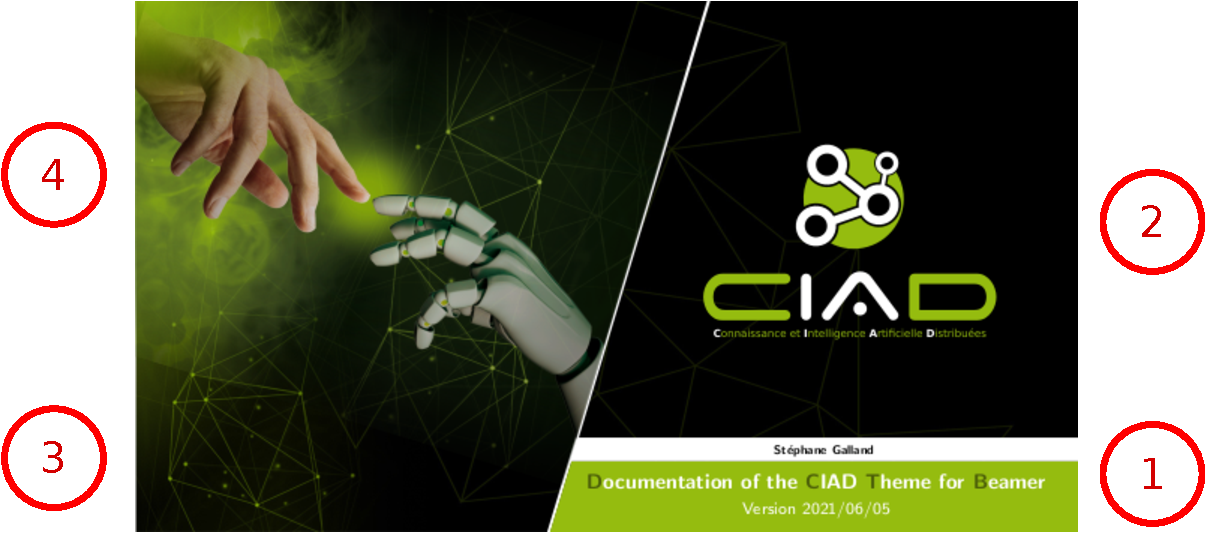
\includegraphics[width=.5\linewidth]{frontpage}
	\end{center}
	\begin{enumerate}
		\item the title of the slides
		\item a picture on the right that could be changed (e.g. the CIAD logo)
		\item a background picture that could be changed (e.g. the black background)
		\item a picture on the left that could be changed (e.g. the hands)
	\end{enumerate}
\end{frame}

\begin{frame}[t]{Change the Right Picture \textcircled{2}}
	For changing the picture on the right \textcircled{2}, use the macro: \\[.25cm]
	\texttt{{\textbackslash}settitlepagerightfigure\{x\}\{y\}\{pgf-id\}} \\[.25cm]
	\begin{itemize}
		\item (\texttt{x}, \texttt{y}) is the coordinate where to put the picture.
		\item \texttt{pgf-id} is the identifier of the picture that is declared with the macro \texttt{{\textbackslash}declarepgfimage[size]\{pgf-id)\}\{filename\}} before calling the macro \texttt{{\textbackslash}settitlepagerightfigure}.
	\end{itemize}
	\begin{example}
		\texttt{{\textbackslash}pgfdeclareimage[width=5cm]\{mypicture\}\{utbmlogo\}} \\
		\texttt{{\textbackslash}settitlepagerightfigure\{250\}\{-30\}\{mypicture\}} \\
		\centering
\includegraphics[width=.25\linewidth]{frontpage2}
	\end{example}
\end{frame}

\begin{frame}[t]{Change the Left Picture \textcircled{4}}
	For changing the picture on the left \textcircled{4}, use the macro: \\[.25cm]
	\texttt{{\textbackslash}settitlepageleftfigure\{x\}\{y\}\{pgf-id\}} \\[.25cm]
	\begin{itemize}
		\item (\texttt{x}, \texttt{y}) is the coordinate where to put the picture.
		\item \texttt{pgf-id} is the identifier of the picture that is declared with the macro \texttt{{\textbackslash}declarepgfimage[size]\{pgf-id)\}\{filename\}} before calling the macro \texttt{{\textbackslash}settitlepageleftfigure}.
	\end{itemize}
	\begin{example}
		\texttt{{\textbackslash}pgfdeclareimage[width=5cm]\{mypicture\}\{utbmlogo\}} \\
		\texttt{{\textbackslash}settitlepageleftfigure\{0\}\{-30\}\{mypicture\}} \\
		\centering
\includegraphics[width=.25\linewidth]{frontpage4}
	\end{example}
\end{frame}

\begin{frame}[t]{Change the Left Background \textcircled{3}}
	\smaller For changing the picture on the left background \textcircled{3}, use the macro: \\[.25cm]
	\texttt{{\textbackslash}settitlepageuserbackground\{pgf-id\}} \\[.25cm]
	\begin{itemize}
		\item \texttt{pgf-id} is the identifier of the picture that is declared with the macro \texttt{{\textbackslash}declarepgfimage[size]\{pgf-id)\}\{filename\}} before calling the macro \texttt{{\textbackslash}settitlepageuserbackground}.
	\end{itemize}
	\alertbox{The left picture is automatically removed when the macro above is invoked}
	\begin{example}
		\texttt{{\textbackslash}pgfdeclareimage[height={\textbackslash}paperheight]\{mypicture\}\{mybackground\}} \\
		\texttt{{\textbackslash}settitlepageuserbackground\{mypicture\}} \\
		\centering
\includegraphics[width=.25\linewidth]{frontpage3}
	\end{example}
\end{frame}

\begin{frame}{{Predefined Backgrounds} for the Title Page State}
	Several background pictures are provided into the CIAD Beamer theme for the position \textcircled{3}. In order to select one of these background, the macro below must be used. The list of predefined background is provided in the following slides. \\[.5cm]
	\texttt{{\textbackslash}setpredefinedtitlepagebackground{\#}} \\[.5cm]
	\begin{itemize}
		\item \texttt{\#} is the number of the predefined background, e.g., "\texttt{1}"
	\end{itemize}
\end{frame}

\begin{frame}{{Predefined Background} 1}
	\centering\texttt{{\textbackslash}setpredefinedtitlepagebackground1} \\[.5cm]
	\fbox{\scalebox{0.5}{\insertpredefinedtitlepagebackground1}}
\end{frame}

\begin{frame}{{Predefined Background} 2}
	\centering\texttt{{\textbackslash}setpredefinedtitlepagebackground2} \\[.5cm]
	\fbox{\scalebox{0.5}{\insertpredefinedtitlepagebackground2}}
\end{frame}

\begin{frame}{{Predefined Background} 3}
	\centering\texttt{{\textbackslash}setpredefinedtitlepagebackground3} \\[.5cm]
	\fbox{\scalebox{0.5}{\insertpredefinedtitlepagebackground3}}
\end{frame}

\begin{frame}{{Predefined Background} 4}
	\centering\texttt{{\textbackslash}setpredefinedtitlepagebackground4} \\[.5cm]
	\fbox{\scalebox{0.5}{\insertpredefinedtitlepagebackground4}}
\end{frame}

\begin{frame}{{Predefined Background} 5}
	\centering\texttt{{\textbackslash}setpredefinedtitlepagebackground5} \\[.5cm]
	\fbox{\scalebox{0.5}{\insertpredefinedtitlepagebackground5}}
\end{frame}

\begin{frame}{{Predefined Background} 6}
	\centering\texttt{{\textbackslash}setpredefinedtitlepagebackground6} \\[.5cm]
	\fbox{\scalebox{0.5}{\insertpredefinedtitlepagebackground6}}
\end{frame}

\begin{frame}{{Predefined Background} 7}
	\centering\texttt{{\textbackslash}setpredefinedtitlepagebackground7} \\[.5cm]
	\fbox{\scalebox{0.5}{\insertpredefinedtitlepagebackground7}}
\end{frame}

\begin{frame}{{Predefined Background} 8}
	\centering\texttt{{\textbackslash}setpredefinedtitlepagebackground8} \\[.5cm]
	\fbox{\scalebox{0.5}{\insertpredefinedtitlepagebackground8}}
\end{frame}

\begin{frame}{{Predefined Background} 9}
	\centering\texttt{{\textbackslash}setpredefinedtitlepagebackground9} \\[.5cm]
	\fbox{\scalebox{0.5}{\insertpredefinedtitlepagebackground9}}
\end{frame}

\begin{frame}{{Other Macros} for Changing the Title Page State}
	For restoring the title page to its default state, the following macros are available: \\[.25cm]
	\begin{itemize}
		\item \texttt{{\textbackslash}setdefaulttitlepageleftfigure}: restore the left picture \textcircled{2} to the default CIAD logo
		\item \texttt{{\textbackslash}removetitlepageleftfigure}: remove any picture at position \textcircled{2}
		\item \texttt{{\textbackslash}removetitlepageuserbackground} remove the user background \textcircled{3} and restore the default background
	\end{itemize}
\end{frame}

\subsection{Authors}

\begin{frame}{Authors}
	\begin{itemize}
	\item Authors are defined with the macro: \\
		\texttt{{\textbackslash}author[short]\{long\}}
		\begin{itemize}
		\item the \texttt{long} list of author is displayed on the front page. You should separate the names with the macro \texttt{{\textbackslash}and}.
		\item the \texttt{short} list of author is displayed inside the foot line of the slides. You \alert{must not separate} the names with the macro \texttt{{\textbackslash}and}.
		\end{itemize}
	\vfill
	\item \alert{Alternatively}, you could define the authors with the macros: \\
		\texttt{{\textbackslash}addauthor[short]\{long\}} \\
		\texttt{{\textbackslash}addauthor*[short]\{long\}}
		\begin{itemize}
		\item Add \textbf{one} author to the list of the authors.
		\item The ``starred'' version applies some visual indicators to the name (underline, etc.) It may be used to indicate the name of the talker for example.
		\end{itemize}
	\end{itemize}
	\vfill
	\alertbox{These macros must be put in the preamble of your document.}
\end{frame}

\begin{frame}{Author Description}
	\begin{itemize}
	\item Authors may be described with additional information (affiliation...): \\
		\texttt{{\textbackslash}authordescription\{description\}}
	\end{itemize}
	\vfill
	\alertbox{This macro must be put in the preamble of your document.}
\end{frame}

\subsection{Keywords, Subject and Abstract}

\begin{frame}{Keywords of the Document}
	\begin{itemize}
	\item You could associate keywords to the document with: \\
		\texttt{{\textbackslash}keywords\{text\}}
	\vspace{1em}
	\item These keywords are automatically put in the properties of the generated PDF file.
	\vspace{1em}
	\item To insert the keywords into your slides, you could use the macro: \\
			\texttt{{\textbackslash}insertkeywords}
	\end{itemize}
	\begin{example}
		\insertkeywords
	\end{example}
\end{frame}

\begin{frame}{Subject of the Document}
	\begin{itemize}
	\item You could associate a subject to the document with: \\
		\texttt{{\textbackslash}subject\{text\}}
	\vspace{1em}
	\item This subject is automatically put in the properties of the generated PDF file.
	\vspace{1em}
	\item To insert the subject into your slides, you could use the macro: \\
			\texttt{{\textbackslash}insertsubject}
	\end{itemize}
	\begin{example}
		\insertsubject
	\end{example}
\end{frame}

\begin{frame}{Abstract of the Document}
	\begin{itemize}
	\item You could put a short summary of the document in the following environment:
		\texttt{{\textbackslash}begin\{abstract\}} \\
		\texttt{This is a summary.} \\
		\texttt{{\textbackslash}end\{abstract\}}
	\vspace{1em}
	\begin{abstract}
		This is a summary.
	\end{abstract}
	\item If you include an abstract, be sure that it is not some long text but just a very short message.
	\end{itemize}
\end{frame}

\subsection{Name of the Event}

\begin{frame}[t]{Name of the Event}
	\begin{block}{Definition of the event name}
		\begin{itemize}
		\item You could specify the name of the event for which the slides are written: \\
			\texttt{{\textbackslash}event[short]\{full\}}
		\item the \texttt{full} name is displayed on the front page.
		\item the \texttt{short} name is displayed inside the foot line of the slides.
		\item Put these macros into the document preamble.
		\end{itemize}
	\end{block}
	\begin{block}{Insert the event name in your slides}
		\begin{itemize}
		\item You could insert the full name of the event with: \\
			\texttt{{\textbackslash}inserteventname}
		\item You could insert the short name of the event with: \\
			\texttt{{\textbackslash}insertshorteventname}
		\end{itemize}
	\end{block}
\end{frame}

\subsection{Name and URL of the Institute}

\begin{frame}{Institute Name}
	\begin{itemize}
	\item You could change the name of the institute with the following macro in the document preamble: \\
		\texttt{{\textbackslash}institute[short]\{full\}}
	\item the \texttt{full} name is displayed on the front page.
	\item the \texttt{short} name is displayed inside the foot line of the slides.
	\vspace{1em}
	\item The default full name is: \\
		{\smaller\insertinstitute}
	\item The default short name is: \insertshortinstitute
	\end{itemize}
\end{frame}

\begin{frame}{Institute URL}
	\begin{itemize}
	\item You could change the URL of the institute with: \\
		\texttt{{\textbackslash}instituteurl\{url\}}
	\vspace{1em}
	\item The default url is: \insertinstituteurl
	\vspace{1em}
	\item To insert the institute's URL, you could use the macro: \\
			\texttt{{\textbackslash}insertinstituteurl}
	\end{itemize}
\end{frame}

%%%%%%%%%%%%%%%%%%%%%%%%%%%%%%%%%%%%%%%%%%%%%%%%%%
\section{Header and Footer Tuning}
\sectionsintoc{2-7}
\sectiontableofcontentslide

\subsection{Headline}

\begin{frame}{Headline}
	\begin{itemize}
	\item CIAD theme provides an headline in which you can change the logo.
	\vfill
	\item You could change this headline with: \begin{itemize}\footnotesize
		\item \texttt{{\textbackslash}useheaderempty}: the headline is empty (no icon).
		\item \texttt{{\textbackslash}useheaderdefault}: the headline is filled with the default value (may be changed with one of the macros on the following slide).
		\end{itemize}
	\end{itemize}
\end{frame}

\begin{frame}{Headline without Logo}
	\begin{itemize}
	\item \texttt{{\textbackslash}useheaderempty}
	\end{itemize}
	\begin{center}
		\fakeslide[]{XyZ}{}
	\end{center}
\end{frame}

\begin{frame}{Headline with the CIAD Logo}
	\begin{itemize}
	\item \texttt{{\textbackslash}useheaderlinewithciadlogo}: the default headline contains the CIAD logo.
	\end{itemize}
	\begin{center}
		\fakeslide[fakeciadlogointitle]{XyZ}{}
	\end{center}
\end{frame}

\begin{frame}{Headline with the UTBM Logo}
	\begin{itemize}
	\item \texttt{{\textbackslash}useheaderlinewithutbmlogo}: the default headline contains the UTBM logo.
	\end{itemize}
	\begin{center}
		\fakeslide[fakeutbmlogointitle]{XyZ}{}
	\end{center}
\end{frame}

\begin{frame}{Headline with the UBE Logo}
	\begin{itemize}
		\item \texttt{{\textbackslash}useheaderlinewithubelogo}: the default headline contains the UBE logo.
	\end{itemize}
	\begin{center}
		\fakeslide[fakeubelogointitle]{XyZ}{}
	\end{center}
\end{frame}

\begin{frame}[t]{Headline with a User-defined Logo}
	\begin{itemize}
	\item \texttt{{\textbackslash}useheaderlinewithuserlogo[options]\{filename\}}: the default headline contains the given image.
	\item Options may be: \begin{itemize}
			\item \texttt{width=<length>} - the width of the image (default: $1$cm);
			\item \texttt{height=<length>} - the height of the image (no default);
			\item \texttt{x=<float>} - the position of the image along x axis (default: $415$);
			\item \texttt{y=<float>} - the position of the image along y axis (default: $-16$).
			\end{itemize}
	\end{itemize}
	\begin{center}
		\fakeslide[fakeuserlogointitle]{XyZ}{}
	\end{center}
\end{frame}

\begin{frame}[t]{Slide Title Coloring}
	\begin{itemize}
	\item By default the title of a slide is rendered with two colors:
		\begin{itemize}
		\item The green color is used for the first part (as shown for the title of this slide); and
		\item The white color is used for the second part.
		\end{itemize}
	\item \emph{By default, only the first word of the title is considered asthe first part of the title (colored in green)}
	\item If you would like to change the words in the first part (colored in green), you could enclose them with braces:
	\item Example:
		\begin{itemize}
		\item The following slide has the title \texttt{This is an example}, and the two first words are colored in white.
		\item The title is written as: \texttt{\{This is\} an example}
		\end{itemize}
	\end{itemize}
\end{frame}

\begin{frame}{{This is} an example}
	Show the previous slide for explaination on this example slide.
\end{frame}

\subsection{Footline}

\begin{frame}[t]{Footline}
	\smaller
	\begin{itemize}
	\item Beamer provides a footline in which the progress of the presentation may be shown.
	In the CIAD theme, this footline is located at the bottom left of the slides.
	\vspace{1em}
	\item You could change this footline with: \begin{itemize}
		\item \texttt{{\textbackslash}usefootlinefortitlepage}: the footline contains the same footline as on the title page.
		\item \texttt{{\textbackslash}usefootlinewithdocumentname}: the footline contains the title of the presentation, and other document informations.
		\item \texttt{{\textbackslash}usefootlinewithsections}: the footline contains the list of the sections of the presentation.
		\end{itemize}
	\vspace{1em}
	\item The following macro is used for inserting the official laboratory logos at the bottom right corner of the slides: \\
		\texttt{{\textbackslash}insertinstitutelogosinfootline\{macros\}}
		\begin{itemize}
		\item The parameter is the set of macros to insert between the logos (basically a spacing macro).
		\item You could redefine this macro for changing the logos.
		\end{itemize}
	\end{itemize}
\end{frame}

\subsection{Partner Logo}

\begin{frame}{Logos for the Partners}
	\begin{itemize}
	\item You could add on all slides one or more logos for your partner(s): \\
		\texttt{{\textbackslash}partnerlogo[options]\{filename\}}
	\item You must call the previous macro for each partner logo.
	\item The \texttt{filename} is the name of the picture.
	\vspace{1em}
	\item This figure is declared with \texttt{{\textbackslash}pgfdeclareimage} with the key ``CIADpartnerlogo''.
	\item The figure could be re-used with \texttt{{\textbackslash}pgfuseimage}.
	\item The \texttt{options} are passed to \texttt{{\textbackslash}pgfdeclareimage}. The default option is \texttt{height=.5cm}.
	\item For removing all the partner logos, use: \texttt{{\textbackslash}nopartnerllogo}.
	\end{itemize}
\end{frame}


\subsection{Frame Numbering}

\begin{frame}{Total Number of Frames}
	\begin{itemize}
	\item The total number of slides in the core part of the presentation could be obtained with: \\
		\texttt{{\textbackslash}inserttotalcoreframenumber}
	\item For example, this documentation document has \inserttotalcoreframenumber\ slides.
	\end{itemize}
\end{frame}

\begin{frame}[label=progressbartypes,t]{Style for the Frame Numbers}
	\begin{itemize}
	\item The following macro changes the style of the frame numbers:
		\begin{itemize}
		\item \texttt{{\textbackslash}insertframenumbering[type number]}
		\item The \texttt{type number} is the identifier of the progress bar to be used:
		\end{itemize}
	\end{itemize}
	\begin{stabularx}{|c|c|X|}
	\tabularhead{Type number}{Output}{Explanation} \\
	\texttt{1} & \insertframenumbering[1] & Show the current frame and its position (in green) in the total number of frames. \\
	\hline
	\texttt{2} & \colorbox{footline.bg}{\tiny\insertframenumbering[2]} & Show the current frame and the total number of frames. \\
	\hline
	\texttt{3} & \insertframenumbering[3] & Same as the type \texttt{1} with a progression bar for the current section (in magenta). \\
	\end{stabularx}
\end{frame}

\subsection{Continuation Text}
\begin{frame}{\subsecname}
	\begin{itemize}
	\item When continuing a frame, Beamer insert the ``continuation text'' after the title.
	\vfill
	\item To insert the continuation text manually, you should use one of:
		\texttt{{\textbackslash}insertcontinuationtext} \\
		\texttt{{\textbackslash}insertcontinuationwith\{integer\}}
	\item The parameter is the value of the continuation counter to display.
	\vfill
	\item \inlineexample{in the following frame, the macro is used in the title \texttt{{\textbackslash}insertcontinuationtext}.}
	\item \inlineexample{in the second following frame, the macro is used in the title \texttt{{\textbackslash}insertcontinuationwith\{34\}}.}
	\end{itemize}
\end{frame}

\begin{frame}{Example of continuation \insertcontinuationtext}
	The continuation text in the title of this frame is given by the macro \texttt{{\textbackslash}insertcontinuationtext}.
\end{frame}

\begin{frame}{Example of continuation \insertcontinuationwith{34}}
	The continuation text in the title of this frame is given by the macro \texttt{{\textbackslash}insertcontinuationwith\{34\}}.
\end{frame}


%%%%%%%%%%%%%%%%%%%%%%%%%%%%%%%%%%%%%%%%%%%%%%%%%%
\section{Background Picture}
\sectionsintoc{3-8}
\sectiontableofcontentslide

\begin{frame}{Changing the Background Picture}
	The CIAD Beamer style is able to add a picture on the background of the slides (below your text). \\[.5cm]
	The following slides explain how to:
	\begin{enumerate}
		\item use one of the pre-defined background pictures
		\item add your own background picture
		\item insert a background picture in your text
		\item select a background picture randomly
	\end{enumerate}
\end{frame}

\subsection{Predefined Background Pictures}

\begin{frame}{Using a Predefined Background Picture}
	\begin{itemize}
		\item For using a predefined background picture, you could define it for all the slides, or for a specific slide \\[.5cm]
		\item For all the slides, you have to the \texttt{background=XX} option to the document class, where \texttt{XX} is the number of the predefined picture \\[.5cm]
		\item For a specific slide, you have to pass the \texttt{background=XX} option to the frame, where \texttt{XX} is the number of the predefined picture
	\end{itemize}
\end{frame}

\begin{frame}[t]{{Pre-defined Background Picture:} 1}
	\texttt{{\textbackslash}documentclass[background=1]\{ciadbeamer\}} \\[.25cm]
	\texttt{{\textbackslash}begin\{frame\}[background=1]} \\[.25cm]
	\centering\fbox{\scalebox{0.5}{\insertslidebackgroundpicture1}} \\[.25cm]
	\alertbox*{This background picture is candidate for random background}
\end{frame}

\begin{frame}[t]{{Changing the Background Picture:} 2}
	\texttt{{\textbackslash}documentclass[background=2]\{ciadbeamer\}} \\[.25cm]
	\texttt{{\textbackslash}begin\{frame\}[background=2]} \\[.25cm]
	\centering\fbox{\scalebox{0.5}{\insertslidebackgroundpicture2}} \\[.25cm]
	\alertbox*{This background picture is candidate for random background}
\end{frame}

\begin{frame}[t]{{Changing the Background Picture:} 3}
	\texttt{{\textbackslash}documentclass[background=3]\{ciadbeamer\}} \\[.25cm]
	\texttt{{\textbackslash}begin\{frame\}[background=3]} \\[.25cm]
	\centering\fbox{\scalebox{0.5}{\insertslidebackgroundpicture3}} \\[.25cm]
	\alertbox*{This background picture is candidate for random background}
\end{frame}

\begin{frame}[t]{{Changing the Background Picture:} 4}
	\texttt{{\textbackslash}documentclass[background=4]\{ciadbeamer\}} \\[.25cm]
	\texttt{{\textbackslash}begin\{frame\}[background=4]} \\[.25cm]
	\centering\fbox{\scalebox{0.5}{\insertslidebackgroundpicture4}} \\[.25cm]
	\alertbox{This background picture cannot be candidate for random background}
\end{frame}

\begin{frame}[t]{{Changing the Background Picture:} 5}
	\texttt{{\textbackslash}documentclass[background=5]\{ciadbeamer\}} \\[.25cm]
	\texttt{{\textbackslash}begin\{frame\}[background=5]} \\[.25cm]
	\centering\fbox{\scalebox{0.5}{\insertslidebackgroundpicture5}} \\[.25cm]
	\alertbox{This background picture cannot be candidate for random background}
\end{frame}

\begin{frame}[t]{{Changing the Background Picture:} 6}
	\texttt{{\textbackslash}documentclass[background=6]\{ciadbeamer\}} \\[.25cm]
	\texttt{{\textbackslash}begin\{frame\}[background=6]} \\[.25cm]
	\centering\fbox{\scalebox{0.5}{\insertslidebackgroundpicture6}} \\[.25cm]
	\alertbox*{This background picture is candidate for random background}
\end{frame}

\begin{frame}[t]{{Changing the Background Picture:} 7}
	\texttt{{\textbackslash}documentclass[background=7]\{ciadbeamer\}} \\[.25cm]
	\texttt{{\textbackslash}begin\{frame\}[background=7]} \\[.25cm]
	\centering\fbox{\scalebox{0.5}{\insertslidebackgroundpicture7}} \\[.25cm]
	\alertbox*{This background picture is candidate for random background}
\end{frame}

\begin{frame}[t]{{Changing the Background Picture:} 8}
	\texttt{{\textbackslash}documentclass[background=8]\{ciadbeamer\}} \\[.25cm]
	\texttt{{\textbackslash}begin\{frame\}[background=8]} \\[.25cm]
	\centering\fbox{\scalebox{0.5}{\insertslidebackgroundpicture8}} \\[.25cm]
	\alertbox{This background picture cannot be candidate for random background}
\end{frame}

\begin{frame}[t]{{Changing the Background Picture:} 9}
	\texttt{{\textbackslash}documentclass[background=9]\{ciadbeamer\}} \\[.25cm]
	\texttt{{\textbackslash}begin\{frame\}[background=9]} \\[.25cm]
	\centering\fbox{\scalebox{0.5}{\insertslidebackgroundpicture9}} \\[.25cm]
	\alertbox*{This background picture is candidate for random background}
\end{frame}

\begin{frame}[t]{{Changing the Background Picture:} 10}
	\texttt{{\textbackslash}documentclass[background=10]\{ciadbeamer\}} \\[.25cm]
	\texttt{{\textbackslash}begin\{frame\}[background=10]} \\[.25cm]
	\centering\fbox{\scalebox{0.5}{\insertslidebackgroundpicture{10}}} \\[.25cm]
	\alertbox*{This background picture is candidate for random background}
\end{frame}


\subsection{Add our Background Pictures}

\begin{frame}{\subsecname}
	Two functions ar provided for adding our own background picture: \\[.25cm]
	\texttt{{\textbackslash}addslidebackgroundpicture[alternatecolor]\{x\}\{y\}\{width\}\{filename\}} \\[.25cm]
	\texttt{{\textbackslash}addslidebackgroundpicture*[alternatecolor]\{x\}\{y\}\{width\}\{filename\}} \\[.25cm]
	\begin{itemize}
		\item (\texttt{x},\texttt{y}) is the position of the background on the slide
		\item \texttt{width} is the width of the picture
		\item \texttt{filename} is the filename of the picture
		\item \texttt{alternatecolor} is a boolean flag that indicates if the alternate colors should be preferred to regular colors when used with this background. Alternate colors are usually considered to be suitable with dark brackground pictures
		\item \emph{The stared version of the macro has the effect to register the picture as a candidate for the random selection of the background}
	\end{itemize}
\end{frame}

\subsection{Insert a Background Picture}

\begin{frame}{\subsecname}
	The following macros enable you to insert the background picture: \\[.25cm]
	\texttt{{\textbackslash}insertslidebackgroundpicture\{num\}} \\[.25cm]
	\texttt{{\textbackslash}putslidebackgroundpicture\{num\}} \\[.25cm]
	\texttt{{\textbackslash}insertcurrentslidebackgroundpicture} \\[.25cm]
	\begin{itemize}
		\item \texttt{num} is the number of the predefined picture
		\item \texttt{{\textbackslash}insertslidebackgroundpicture} is replaced by the picture, using PGF API
		\item \texttt{{\textbackslash}putslidebackgroundpicture} places the picture at the expected position in the enclosing Tikz environment
		\item \texttt{{\textbackslash}insertcurrentslidebackgroundpicture} places the current picture at the expected position in the enclosing Tikz environment; the current picture depends on the "\texttt{background}" configuration and the random selection of the picture
	\end{itemize}
\end{frame}

\subsection{Random Background Picture}

\begin{frame}{\subsecname}
	It is possible to change the background picture random. The candidates are those added with the \texttt{{\textbackslash}addslidebackgroundpicture*} macro \\[.25cm]
	Turning on the random selection of the background is done by specifying the value "\texttt{randombackground}" as class option: \\[.25cm]
	\texttt{{\textbackslash}documentclass[randombackground]\{ciadbeamer\}}
\end{frame}

\subsection{Background Picture for Outline Slides}

\begin{frame}{\subsecname}
	The following function is provided for changing the background picture for the outline slides: \\[.25cm]
	\texttt{{\textbackslash}addslidebackgroundpictureO[alternatecolor]\{x\}\{y\}\{width\}\{filename\}} \\[.25cm]
	\begin{itemize}
		\item (\texttt{x},\texttt{y}) is the position of the background on the slide
		\item \texttt{width} is the width of the picture
		\item \texttt{filename} is the filename of the picture
		\item \texttt{alternatecolor} is a boolean flag that indicates if the alternate colors should be preferred to regular colors when used with this background. Alternate colors are usually considered to be suitable with dark brackground pictures
	\end{itemize}
\end{frame}



%%%%%%%%%%%%%%%%%%%%%%%%%%%%%%%%%%%%%%%%%%%%%%%%%%
\section{Sectionning}
\sectionsintoc{4-}
\sectiontableofcontentslide

\subsection{Table of Contents}

\begin{frame}{Table of Contents/Outline}
	\begin{itemize}
	\item The CIAD theme provides a convenient macro to insert a table of contents into a slide: \\
		\texttt{{\textbackslash}tableofcontentsslide[toc options][frame options]}
	\vspace{1em}
	\item It is equivalent to: \\
		\texttt{{\textbackslash}begin\{frame\}[t,frame options]} \\
		\texttt{{\textbackslash}frametitle\{{\textbackslash}translate\{Outline\}\}} \\
		\texttt{{\textbackslash}tableofcontents[toc options]} \\
		\texttt{{\textbackslash}end\{frame\}}
	\vspace{1em}
	\item In addition to the standard options for {{\textbackslash}tableofcontents}, the option \texttt{onlyparts} permits to display the list of the parts, only.
	\end{itemize}
\end{frame}

\begin{frame}{Table of Contents for Sections}
	\begin{itemize}
	\item The CIAD theme provides convenient macros for showing the TOC for sections into a slide: \\
		\texttt{{\textbackslash}sectiontableofcontentslide} \\
		\texttt{{\textbackslash}subsectiontableofcontentslide} \\
		\texttt{{\textbackslash}subsubsectiontableofcontentslide}
	\item They provide standard show/hide configurations for each section type.
	\item You could control the list of the sections that are shown in the TOC by specifying a range of section numbers with: \\
		\texttt{{\textbackslash}sectionsintoc\{section\_range\}} \\
		It is equivalent to passing option \texttt{sections={section\_range}} to the \texttt{{\textbackslash}tableofcontent} command
	\item The \texttt{{\textbackslash}sectionsintoc} macro is active until it is evaluated again or the following resetting macro is used: \\
		\texttt{{\textbackslash}resetsectionsintoc}
	\end{itemize}
\end{frame}

\subsection{Part Sectioning}

\begin{frame}{Part Sectioning}
	\begin{itemize}
	\item The CIAD theme provides specific implementations of the \texttt{{\textbackslash}part} macro: \\
		\texttt{{\textbackslash}part[options]\{title\}} \\
		\texttt{{\textbackslash}part*[options]\{title\}}
	\vfill
	\item Options may be: \begin{itemize}
		\item a string value that is the ``short'' title of the part that is appearing in the table of contents.
		\item the pair \texttt{title=text} to define the ``short'' title.
		\item the pair \texttt{author=text} to define the author of the part.
		\item the pair \texttt{label=id} to define the label of the part.
		\end{itemize}
	\vfill
	\item The stared version of \texttt{{\textbackslash}part} does not add the part in the table of contents.
	\end{itemize}
\end{frame}

\begin{frame}{{Changing the prefix} in the part's slides}
	\begin{itemize}
	\item By default, each part starts with a slide with only the part's title on, without a prefix such as ``Chapter X''.
	\vfill
	\item The CIAD theme provides the following macros to change the part's prefix:
		\begin{itemize}
		\item \texttt{{\textbackslash}insertpartprefix} insert the current part prefix.
		\item \texttt{{\textbackslash}partprefix[counter text]\{text\}} changes the prefix to ``text'' followed by ``counter text''.
		\item \texttt{{\textbackslash}resetpartprefix} resets the prefix to the empty text.
		\end{itemize}
	\end{itemize}
	\vfill
	\begin{example}
		\texttt{{\textbackslash}partprefix[{\textbackslash}arabic\{part\}]\{Chapter\}} \\
		produces: ``Chapter 1'', ``Chapter 2'', \dots
	\end{example}
\end{frame}

\subsection{Limit sections in TOC}

\begin{frame}{{Limit Sections} in TOC}
	\begin{itemize}
	\item Sometimes the number of sections into the TOC is too high for enabling to show all the sections' titles on the slide.
	\item It is possible to specifiy a range of section numbers that should appear on the TOC slide. The new optional argument \texttt{<>} of \texttt{{\textbackslash}section}: \\
		\texttt{{\textbackslash}section<range>[title in toc]\{title\}} \\
		\texttt{{\textbackslash}section*<range>[title in toc]\{title\}} \\
		\texttt{{\textbackslash}section<range>*[title in toc]\{title\}}
	\vfill
	\item Arguments are: \begin{itemize}
		\item \texttt{range}: the range of section numbers to show on the TOC.
		\item \texttt{title in toc}: the title of the section into the TOC.
		\item \texttt{title}: the standard title of the section.
		\end{itemize}
	\item The `'starred'' macros above ignore the \texttt{title in toc} argument and do not add the section into the TOC.
	\end{itemize}
\end{frame}

\subsection{Appendix}

\begin{frame}{\subsecname}
	\begin{itemize}
	\item The CIAD theme supports the appendix part.
	\vspace{1em}
	\item To create the appendix, you must:
		\begin{enumerate}
		\item put the macro \texttt{{\textbackslash}appendix} in your {\TeX} file; or
		\item put the macro \texttt{{\textbackslash}bibliography} in your {\TeX} file.
		\end{enumerate}
	\vspace{1em}
	\item All the slides that are put after the creation of the appendix are assumed to be part of the appendix.
	\item The slides in the appendix are not considered in the total number of slides for the core part of the document (see \texttt{{\textbackslash}inserttotalcoreframenumber}).
	\item The slide numbers in the appendix are roman (not arabic), and the page counter is reset at the begining of the appendix.
	\end{itemize}
\end{frame}

\subsection{Bibliography}

\begin{frame}{Bibliography}
	\begin{itemize}
	\item You are able to include a bibliography in your slides with the two standard {\LaTeX} macros: \\
		\texttt{{\textbackslash}bibliographystyle\{style\}} \\
		\texttt{{\textbackslash}bibliography\{filename\}}
	\vspace{1em}
	\item If you do not call \texttt{{\textbackslash}bibliographystyle}, the default style is \texttt{apalike}.
	\vspace{1em}
	\item When the macro \texttt{{\textbackslash}bibliography} is used, the appendix section is started if it was not already done.
	\item The bibliography slides are \alert{always at the end of the document}. Even if you put slides after the {\textbackslash}bibliography macro.
	\item \emph{The first slide of the bibliography is marked with the label ``\texttt{bibliographyslide}'' for \texttt{{\textbackslash}hyperlink}.}
	\end{itemize}
\end{frame}

%%%%%%%%%%%%%%%%%%%%%%%%%%%%%%%%%%%%%%%%%%%%%%%%%%
\section{Special Slides}
\sectionsintoc{5-}
\sectiontableofcontentslide

\subsection{Slide for titles}

\begin{frame}{\subsecname}
	\begin{itemize}
	\item Slide that is drawn as a ``part'' frame but \emph{without adding a part section in the document}. This command is usually used for showing the frame outside the context of a \texttt{{\textbackslash}part} command.
	\item \LaTeX\ Command:\\
		\texttt{{\textbackslash}partframeonly\{title\}}
	\item \texttt{title} is the title that must be shown on the frame
	\end{itemize}
	\vspace{1cm}
	Example sohwn on next slide: \\
	\texttt{{\textbackslash}partframeonly\{This is an example of partframeonly\}}
\end{frame}

\partframeonly{This is an example of partframeonly}

\subsection{Slide with a Right Title}

\begin{frame}{\subsecname}
	\begin{itemize}
	\item Slide that contains an additional title on the right, and the standard content is rendered on the left part of slide.
	\item Definition with the following environment: \\
		\texttt{{\textbackslash}begin\{righttitleframe\}[options]\{main title\}\{right title\}} \\
		\texttt{Content of the Slide} \\
		\texttt{{\textbackslash}end\{righttitleframe\}}
	\item \texttt{options} are options to pass to the frame
	\item \texttt{main title} is the title to be rendered at the top of the frame
	\item \texttt{right title} is the title to be rendered at the right of the frame
	\end{itemize}
\end{frame}

\begin{righttitleframe}{Example of frame with right title}{This is the right title}
	This is the standard frame content. See the previous slide for an explanation.
\end{righttitleframe}

\subsection{Slide with Text and Picture}

\begin{frame}{Slide with Text and Picture}
	\begin{itemize}
		\item Slide with a regular text area on the left and a picture inside a big green area on the right.
		\item Definition with the following environment: \\
		\texttt{{\textbackslash}begin\{textpictureframe\}[options]\{main title\}\{pgf-id\}} \\
		\texttt{Content of the Slide} \\
		\texttt{{\textbackslash}end\{textpictureframe\}}
		\item \texttt{options} are options to pass to the frame
		\item \texttt{main title} is the title to be rendered at the top of the frame
		\item \texttt{pgf-id} is identifier of an image that was declared with the \texttt{{\textbackslash}addtextpicturepicture}: \\
		\texttt{{\textbackslash}addtextpicturepicture\{pgf-id\}\{picture filename\}} \\
		\texttt{{\textbackslash}addtextpicturepicture*\{pgf-id\}\{picture filename\}}
		no-star version forces the width size of the picture; star version forces the height size of the picture
	\end{itemize}
\end{frame}

\addtextpicturepicture{tpexample1}{ciad-title-background-left9}
\begin{textpictureframe}{{Example of frame} with left text and right picture}{tpexample1}
	This is the standard frame content. See the previous slide for an explanation. \\[.5cm]
	\smaller
	\texttt{{\textbackslash}addtextpicturepicture\{tpexample1\} \{ciad-title-background-left9\}} \\
	\texttt{{\textbackslash}begin\{textpictureframe\} \{Example of frame with left text and right picture\}\{tpexample1\}} \\
	\texttt{{\textbackslash}end\{textpictureframe\}}
\end{textpictureframe}

\subsection{Slide with Lawn}

\begin{frame}{Slide with a lawn on the left}
	\begin{itemize}
		\item Slide that a green area (the lawn) on which text is displayed, and a picture is drawn on the right of the lawn.
		\item Definition with the following environment: \\
		\texttt{{\textbackslash}begin\{leftlawnframe\}[options]\{main title\}\{pgf-id\}} \\
		\texttt{Content of the Slide} \\
		\texttt{{\textbackslash}end\{leftlawnframe\}}
		\item \texttt{options} are options to pass to the frame
		\item \texttt{main title} is the title to be rendered at the top of the frame
		\item \texttt{pgf-id} is identifier of an image that was declared with the \texttt{{\textbackslash}addlawnpicture}: \\
		\texttt{{\textbackslash}addlawnpicture\{pgf-id\}\{picture filename\}} \\
		\texttt{{\textbackslash}addlawnpicture*\{pgf-id\}\{picture filename\}}
		no-star version forces the width size of the picture; star version forces the height size of the picture
	\end{itemize}
\end{frame}

\addlawnpicture{lawnexample1}{ciad-title-background-left9}
\begin{leftlawnframe}{{Example of frame} with left lawn}{lawnexample1}
	This is the standard frame content. See the previous slide for an explanation. \\[.5cm]
	\smaller
	\texttt{{\textbackslash}addlawnpicture\{ lawnexample1\} \{ciad-title-background-left9\}} \\
	\texttt{{\textbackslash}begin\{leftlawnframe\} \{Example of frame with left lawn\}\{lawnexample1\}} \\
	\texttt{{\textbackslash}end\{leftlawnframe\}}
\end{leftlawnframe}

\begin{frame}{Slide with a lawn on the right}
	\begin{itemize}
		\item Slide that a green area (the lawn) on which text is displayed, and a picture is drawn on the left of the lawn.
		\item Definition with the following environment: \\
			\texttt{{\textbackslash}begin\{rightlawnframe\}[options]\{main title\}\{pgf-id\}} \\
			\texttt{Content of the Slide} \\
			\texttt{{\textbackslash}end\{rightlawnframe\}}
		\item \texttt{options} are options to pass to the frame
		\item \texttt{main title} is the title to be rendered at the top of the frame
		\item \texttt{pgf-id} is identifier of an image that was declared with the \texttt{{\textbackslash}addlawnpicture}: \\
		\texttt{{\textbackslash}addlawnpicture\{pgf-id\}\{picture filename\}} \\
		\texttt{{\textbackslash}addlawnpicture*\{pgf-id\}\{picture filename\}} \\
		no-star version forces the width size of the picture; star version forces the height size of the picture
	\end{itemize}
\end{frame}

\begin{rightlawnframe}{{Example of frame} with right lawn}{lawnexample1}
	This is the standard frame content. See the previous slide for an explanation. \\[.5cm]
	\smaller
	\texttt{{\textbackslash}addlawnpicture\{ lawnexample1\} \{ciad-title-background-left9\}} \\
	\texttt{{\textbackslash}begin\{rightlawnframe\} \{Example of frame with right lawn\}\{lawnexample1\}} \\
	\texttt{{\textbackslash}end\{rightlawnframe\}}
\end{rightlawnframe}

\subsection{Slide with a Grid of Icons}

\begin{frame}[t]{Slide with a Grid of Icons}
	\begin{itemize}
		\item Slide has a grid structure with 10 cells
		\item Each cell contains an icon and a text
			\begin{center}
				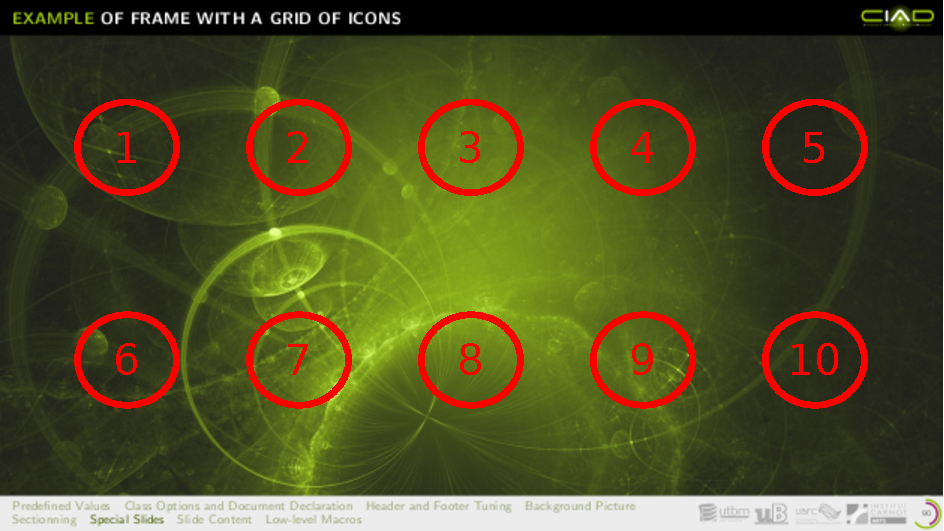
\includegraphics[width=.5\linewidth]{gridframe}
			\end{center}
		\item Definition with the following environment: \\
			\texttt{{\textbackslash}begin\{gridframe\}[options]\{main title\}} \\
			\emph{Cell declarations (see next slide)} \\
			\texttt{{\textbackslash}end\{gridframe\}}
	\end{itemize}
\end{frame}

\begin{frame}{{Declaration of a cell} into the icon grid}
	The declaration of a cell into the icon grid is possible by using one of the two following commands
	\begin{block}{Declaration of a cell with a picture \Emph{loaded by PGF}}
		\texttt{{\textbackslash}cell\{cell-number\}\{pgf-id\}\{text\}} \\[.25cm]
		Each picture must be declared with the following command in order to be loadable by PGF: \\
			\texttt{{\textbackslash}addgridpicture\{pgf-id\}\{picture-filename\}}
	\end{block}
	\begin{block}{Declaration of a cell with a picture \Emph{loaded by Graphicx}}
		\texttt{{\textbackslash}cell*\{cell-number\}\{picture-filename\}\{text\}}
	\end{block}
\end{frame}

\resolvepicturename{example3}
\addgridpicture{example3}{\resolvedfilename}
\begin{gridframe}{{Example of frame} with a grid of icons}
	\cell*2{example1}{Cell 2}
	\cell*3{example2}{Cell 3}
	\cell4{example3}{Cell 4}
	\cell*6{example4}{Cell 6}
	\cell*8{example5}{Cell 8}
	\cell*{10}{example6}{Cell 10}
\end{gridframe}

\begin{gridframe}[background=4,c]{{Example of frame} with a grid of icons \insertcontinuationtext}
	\cell*2{example1}{Cell 2}
	\cell*3{example2}{Cell 3}
	\cell4{example3}{Cell 4}
	\cell*6{example4}{Cell 6}
	\cell*8{example5}{Cell 8}
	\cell*{10}{example6}{Cell 10}
\end{gridframe}

\subsection{Slide with a Single Figure}

\begin{frame}{Slide with a Single Figure}
	\begin{itemize}
	\item The CIAD theme provides a macro that permits to display a picture on the entire slide: \\
			\texttt{{\textbackslash}figureslide[options]\{Title of the slide\}\{file\}}
	\item The size of the picture is adjusted to the slide drawing area.
	\item Example: \texttt{{\textbackslash}figureslide\{XyZ\}\{ciadlogo\}} 
	\end{itemize}
	\vspace{1em}
	\begin{center}
		\fakeslide{XyZ}{
			\put(-3,20){
\includegraphics[width=\linewidth]{ciadlogo}}
		}
	\end{center}
\end{frame}

\begin{frame}{Slide with a Single Figure \insertcontinuationtext}
	\begin{itemize}
	\item Options for \texttt{{\textbackslash}figureslide} are:
		\begin{itemize}
		\item \texttt{width=<length>}, specifies the width of the image.
		\vfill
		\item \texttt{height=<length>}, specifies the height of the image.
		\vfill
		\item \texttt{scale=<float>}, specifies the scaling factor of the image.
		\vfill
		\item \texttt{valign=t|c|b}, specifies the vertical alignment of the image (\texttt{t}: top, \texttt{c}: center, \texttt{b}: bottom).
		\vfill
		\item \texttt{halign=l|c|r}, specifies the horizontal alignment of the image (\texttt{l}: left, \texttt{c}: center, \texttt{r}: right).
		\vfill
		\item \texttt{label=<text>}, specifies the label for the frame.
		\vfill
		\item \texttt{subtitle=<text>}, specifies the subtitle for the frame.
		\end{itemize}
	\end{itemize}
\end{frame}

\figureslide{Example of a Single Figure on a Slide}{ciadlogo}

\begin{frame}{Slide with a Single ANIMATED Figure}
	\begin{itemize}
	\item The AutoLaTeX\footnote{\url{http://www.arakhne.org/autolatex}} tool provides a \LaTeX\ package that enables to include images with layers. Each layers may be displayed in a separate frame by Beamer.
	\vfill
	\item If you have included the AutoLaTeX package, the following macro enables you to display an animated figure on the entire space of a slide: \\
		\texttt{{\textbackslash}animatedfigureslide<framespec>[options]\{title\}\{file\}}
	\item This macro is similar to \texttt{{\textbackslash}figureslide}, except that the given picture must be displayable by the macro \texttt{{\textbackslash}includeanimatedfigure}, provided by AutoLaTeX.
	\end{itemize}
\end{frame}

\begin{frame}{How to Create an ANIMATED Figure?}
	\smaller
	\alertbox{You must use the AutoLaTeX\footnote{\url{http://www.arakhne.org/autolatex}} tool.}
	\begin{enumerate}
	\item Open your favorite SVG editor (Inkscape, etc.).
	\item Create the SVG figure with a layer for each frame.
	\item Put the frame specification into the names of the layers. The frame specification gives the frame numbers for which the SVG layer is displayed. \inlineexample{\texttt{<1-3>} indicates the frames 1 to 3. Do not forget to put the lower-than and upper-than symbols.}
	\item Save and run AutoLaTeX. This tool will create a PDF file for each layer, and a \TeX\ file that is controlling the displaying of the figure.
	\item Include the figure with: \texttt{{\textbackslash}includeanimatedfigure<framespec>[options]\{texfilename\}} or with \texttt{{\textbackslash}animatedfigureslide}.
	\end{enumerate}
\end{frame}

\begin{frame}{Example of ANIMATED Figure}
	\begin{itemize}
	\item Three layers are defined with the following names:
		\begin{itemize}
		\item \texttt{Layer1 <1->} --- display the circle in all the frames, starting from the first.
		\item \texttt{Layer2 <2>} --- display the top yellow star in the second frame.
		\item \texttt{Layer3 <3>} --- display the right yellow star in the third frame.
		\end{itemize}
	\end{itemize}
	% The following code is a copy paste of the \includeanimatedfigure given by AutoLaTeX.
	\begin{center}
		\resizebox{.3\linewidth}{!}{
			\resolvepicturename{layerexample}
			\input{\resolvedfilename}
		}
	\end{center}
\end{frame}

\begin{frame}{Slide with a Single Embedded Video}
	\begin{itemize}
	\item The CIAD theme provides a macro that permits to display a \emph{embedded video} on the entire slide. This video could be displayed during the show with a viewer such as PDFPC: \\
		\texttt{{\textbackslash}embeddedvideoslide[options]\{Title of the slide\}\{video file\}\{image file\}}
	\item The size of the picture is adjusted to the slide drawing area.
	\item Example: \texttt{{\textbackslash}embeddedvideoslide\{XyZ\}\{myvideo\}\{ciadlogo\}} 
	\item The given image is displayed if the viewer cannot show up the video.
	\end{itemize}
\end{frame}

\begin{frame}{Slide with a Single Embedded Video \insertcontinuationtext}
	\begin{itemize}
	\item Options for \texttt{{\textbackslash}embeddedvideoslide} are:
		\begin{itemize}
		\item \texttt{width=<length>}, specifies the width of the video.
		\vfill
		\item \texttt{height=<length>}, specifies the height of the video.
		\vfill
		\item \texttt{scale=<float>}, specifies the scaling factor of the video.
		\vfill
		\item \texttt{valign=t|c|b}, specifies the vertical alignment of the video (\texttt{t}: top, \texttt{c}: center, \texttt{b}: bottom).
		\vfill
		\item \texttt{halign=l|c|r}, specifies the horizontal alignment of the video (\texttt{l}: left, \texttt{c}: center, \texttt{r}: right).
		\vfill
		\item \texttt{label=<text>}, specifies the label for the frame.
		\vfill
		\item \texttt{subtitle=<text>}, specifies the subtitle for the frame.
		\end{itemize}
	\end{itemize}
\end{frame}

\subsection{Final Slide}

\begin{frame}{{A Slide} at the End}
	\begin{itemize}
	\item The CIAD theme automatically adds a slide at the end of the presentation to avoid ``black'' screen.
	\vfill
	\item The default text on this slide is: ``\translate{Thanks}''.
	\item An other text that is available is: ``\translate{Questions}''.
	\item The third option is to repeat the title slide.
	\vfill
	\item The class options \texttt{thanksslide}, \texttt{questionslide} and \texttt{repeattitleslide} permit to select one of these possibilities.
	\vfill
	\item The macro \texttt{{\textbackslash}finalslidetext\{text\}} may be used to set the text by hand.
	\vfill
	\item \emph{This slide is marked with the label \texttt{finalslide} for \texttt{{\textbackslash}hyperlink}.}
	\vfill
	\item You could display this slide at any moment with: \texttt{{\textbackslash}thanksslide}.
	\end{itemize}
\end{frame}

\subsection{Book Description}

\begin{frame}{Book Description}
	\begin{itemize}
	\item You are able to include a description of a book in your presentation with the macro: \\
		\texttt{{\textbackslash}libraryslide[options]\{picture\}} \\
		\texttt{\{title\}\{authors\}\{How published\}\{ISBN\}}
	\vspace{1em}
	\item The macro creates a slide for a book.
	\vspace{1em}
	\item The \texttt{options} may be composed of pairs of name-value:
		\begin{itemize}
		\item \texttt{frametitle=text}: specifies the title of the frame.
		\item \texttt{subtitle=text}: specifies the subtitle of the book.
		\end{itemize}
	\item If a name is not specified in the options, the ``\texttt{subtitle}'' name is assumed.
	\end{itemize}
\end{frame}

%%%%%%%%%%%%%%%%%%%%%%%%%%%%%%%%%%%%%%%%%%%%%%%%%%
\section{Slide Content}
\sectionsintoc{6-}
\sectiontableofcontentslide

\subsection{{\textbackslash}includegraphics}
\subsectiontableofcontentslide

\begin{frame}{{\textbackslash}includegraphics}
	\alertbox{The macro \textbf{{\textbackslash}includegraphics} is overridden by the theme.}
	\begin{itemize}
	\vspace{2em}
	\item If you don't specify any optional parameter related to the size of the picture in the document, the \textbf{{\textbackslash}includegraphics} macro will use by default: \\
		\textbf{width={\textbackslash}linewidth}
	\end{itemize}
\end{frame}

\subsection{Drawing}
\subsectiontableofcontentslide

\begin{frame}{Put at an Absolute Position}
	\begin{itemize}
	\item If you want to put something at an absolute position in your frame, you could use: \\
		\texttt{{\textbackslash}putat<framespec>(x,y)\{something\}}
	\item \alert{Caution: The added elements are put less deeper than the slide text.}
	\item For putting the elements more deeper than the slide text, use: \\
		\texttt{{\textbackslash}putat*<framespec>(x,y)\{something\}}
	\vspace{1em}
	\item Example: \\
		\texttt{{\textbackslash}putat(180,-20)\{{\textbackslash}color\{red\}\{TESTING\}\}}
	\end{itemize}
	\putat(180,-20){\color{red}{TESTING}}
\end{frame}

\subsection{Blocks}
\subsectiontableofcontentslide

\begin{frame}{Left-Anchor Block}
	\begin{itemize}
		\item The CIAD Beamer theme provides an environment named ``left-anchor block'' that provides a fancy display for a block of information: \\[.25cm]
			\begin{leftanchorblock}{The title}{XX}
				This is a content
			\end{leftanchorblock}
		\vspace{.5cm}
		\item This type of block has a title, a text to write in the circle (e.g., \texttt{XX}), and a content
		\item The environment for rendering a left-anchor block is: \\[.25cm]
			\texttt{{\textbackslash}begin\{leftanchorblock\}[width]\{title\}\{text in the circle\}} \\
			\mbox{}\hspace{.2cm}\texttt{the content of the block} \\
			\texttt{{\textbackslash}end\{leftanchorblock\}}
	\end{itemize}
\end{frame}

\begin{frame}{Right-Anchor Block}
	\begin{itemize}
		\item The CIAD Beamer theme provides an environment named ``right-anchor block'' that provides a fancy display for a block of information: \\[.25cm]
		\begin{rightanchorblock}{The title}{XX}
			This is a content
		\end{rightanchorblock}
		\vspace{.5cm}
		\item This type of block has a title, a text to write in the circle (e.g., \texttt{XX}), and a content
		\item The environment for rendering a right-anchor block is: \\[.25cm]
		\texttt{{\textbackslash}begin\{rightanchorblock\}[width]\{title\}\{text in the circle\}} \\
		\mbox{}\hspace{.2cm}\texttt{the content of the block} \\
		\texttt{{\textbackslash}end\{rightanchorblock\}}
	\end{itemize}
\end{frame}

\begin{frame}{Mixing Anchor Blocks}
	\begin{leftanchorblock}[.5\linewidth]{The title}{1}
		This is a box with half width
	\end{leftanchorblock}
	\vspace{.5cm}
	\begin{rightanchorblock}{The title}{2}
		This is a content with total width
	\end{rightanchorblock}
\end{frame}

\begin{frame}{Mixing Anchor Blocks \insertcontinuationtext}
	\begin{leftanchorblock}{The title}{1}
		This is a box with total width
	\end{leftanchorblock}
	\vspace{.5cm}
	\begin{rightanchorblock}[.5\linewidth]{The title}{2}
		This is a content with half width
	\end{rightanchorblock}
\end{frame}

\begin{frame}{Multiple Anchor Blocks}
	\begin{columns}
		\begin{column}{.5\linewidth}
			\begin{leftanchorblock}{Title 1}{1}
				Text 1
			\end{leftanchorblock}
			\vspace{.5cm}
			\begin{leftanchorblock}{Title 2}{2}
				Text 2
			\end{leftanchorblock}
		\end{column}
		\begin{column}{.5\linewidth}
			\begin{rightanchorblock}{Title 3}{3}
				Text 3
			\end{rightanchorblock}
			\vspace{.5cm}
			\begin{rightanchorblock}{Title 4}{4}
				Text 4
			\end{rightanchorblock}
		\end{column}
	\end{columns}
\end{frame}

\begin{frame}{Sequence of Right Arrows}
	The CIAD theme defines a sequence of right arrows as:
	\begin{rightarrowsequence}
		\arrow{Arrow 1}
		\arrow[bg=blue]{Arrow 2}
		\arrow{Arrow 3}
		\arrow[bg=red]{Arrow 4}
	\end{rightarrowsequence} \\[.5cm]
	This sequence is obtained by using the following environment: \\
	\texttt{{\textbackslash}begin\{rightarrowsequence\}[g\_options]} \\
	\hspace{.5cm}\texttt{{\textbackslash}arrow[a\_options]\{text\}} \\
	\texttt{{\textbackslash}end\{rightarrowsequence\}}
	
	\begin{itemize}
	\item Each arrow is drawn by the macro \texttt{{\textbackslash}arrow}
	\item \texttt{g\_options} are the options applied to all the arrows (explained on later slide)
	\item \texttt{a\_options} are the options applied to a specific arrow (explained on later slide)
	\end{itemize}
\end{frame}

\resolvepicturename{example1}
\pgfdeclareimage[width=2cm]{arrow-decoration-example1}{\resolvedfilename}
\begin{frame}{Decorations for Right Arrows}
	\smaller
	Each arrow could have a decoration, as illustrated by:
	\begin{rightarrowsequence}
		\arrow[decoration={arrow-decoration-example1}]{Arrow 1}
		\arrow[bg=blue]{Arrow 2}
		\arrow{Arrow 3}
		\arrow[bg=red,fg=blue,decoration={arrow-decoration-example1}]{Arrow 4}
	\end{rightarrowsequence} \\[.5cm]
	This sequence is obtained by: \\
	\texttt{{\textbackslash}begin\{rightarrowsequence\}} \\
	\hspace{.5cm}\texttt{{\textbackslash}arrow[decoration=\{image\}]\{Arrow 1\}} \\
	\hspace{.5cm}\texttt{{\textbackslash}arrow[bg=blue]\{Arrow 2\}} \\
	\hspace{.5cm}\texttt{{\textbackslash}arrow\{Arrow 3\}} \\
	\hspace{.5cm}\texttt{{\textbackslash}arrow[bg=red,fg=blue,decoration=\{image\}]\{Arrow 4\}} \\
	\texttt{{\textbackslash}end\{rightarrowsequence\}}
\end{frame}

\begin{frame}{{Right-Arrow-Sequence} Global Options}
	\begin{itemize}
	\item \texttt{width=\ensuremath{<}length\ensuremath{>}}: width of the sequence (default: \the\linewidth)
	\item \texttt{height=\ensuremath{<}length\ensuremath{>}}: height of the sequence (default: max height of the internal arrows)
	\item \texttt{arrowwidth=\ensuremath{<}length\ensuremath{>}}: default width for the arrows (default: adjusted width depending on the width of the sequence)
	\item \texttt{sep=\ensuremath{<}length\ensuremath{>}}: distance between the arrows
	\item \texttt{topsep=\ensuremath{<}length\ensuremath{>}}: margin at the top of the sequence
	\item \texttt{bottomsep=\ensuremath{<}length\ensuremath{>}}: margin at the bottom of the sequence
	\item \texttt{decorationsep=\ensuremath{<}length\ensuremath{>}}: distance between the decoration (usually an icon) and the text inside an arrow
	\end{itemize}
\end{frame}

\begin{frame}{{Right-Arrow-Sequence} Global Options \insertcontinuationtext}
	\begin{itemize}
	\item \texttt{bg=\ensuremath{<}color\ensuremath{>}}: default background color for all the arrow (default: black)
	\item \texttt{fg=\ensuremath{<}color\ensuremath{>}}: default text color for all the arrow (default: white)
	\end{itemize}
\end{frame}

\begin{frame}{{Right-Arrow-Sequence} Arrow Options}
	\begin{itemize}
	\item \texttt{width=\ensuremath{<}length\ensuremath{>}}: width of the arrow, override the global option
	\item \texttt{bg=\ensuremath{<}color\ensuremath{>}}: background color, override the global option
	\item \texttt{fg=\ensuremath{<}color\ensuremath{>}}: text color, override the global option
	\item \texttt{decoration=\ensuremath{<}id\ensuremath{>}}: identifier if the picture loadable with \texttt{{\textbackslash}pgfuseimage}
	\end{itemize}
\end{frame}

\begin{frame}[t]{Sequence of Bottom Arrows}
	\begin{columns}
		\begin{column}{.2\linewidth}
			\begin{bottomarrowsequence}
				\arrow{Arrow 1}
				\arrow[bg=blue]{Arrow 2}
				\arrow{Arrow 3}
				\arrow[bg=red]{Arrow 4}
			\end{bottomarrowsequence} \\[.5cm]
		\end{column}
		\begin{column}{.8\linewidth}
			The CIAD theme defines a sequence of bottom arrows as:
			\vspace{.5cm}
			This sequence is obtained by using the following environment: \\
			\texttt{{\textbackslash}begin\{bottomarrowsequence\}[g\_options]} \\
			\hspace{.5cm}\texttt{{\textbackslash}arrow[a\_options]\{text\}} \\
			\texttt{{\textbackslash}end\{bottomarrowsequence\}}
			
			\begin{itemize}
			\item Each arrow is drawn by the macro \texttt{{\textbackslash}arrow}
			\item \texttt{g\_options} are the options applied to all the arrows (explained on later slide)
			\item \texttt{a\_options} are the options applied to a specific arrow (explained on later slide)
			\end{itemize}
		\end{column}
	\end{columns}
\end{frame}

\resolvepicturename{example1}
\pgfdeclareimage[width=0.5cm]{bottomarrowexample1}{\resolvedfilename}
\begin{frame}[t]{Decorations for Bottom Arrows}
	\begin{columns}
		\begin{column}{.2\linewidth}
			\begin{bottomarrowsequence}
				\arrow[decoration={bottomarrowexample1}]{Arrow 1}
				\arrow[bg=blue]{Arrow 2}
				\arrow{Arrow 3}
				\arrow[bg=red,fg=blue,decoration={bottomarrowexample1}]{Arrow 4}
			\end{bottomarrowsequence}
		\end{column}
		\begin{column}{.8\linewidth}
			Each arrow could have a decoration, as illustrated by:
			\vspace{.5cm}
			This sequence is obtained by: \\
			\texttt{{\textbackslash}begin\{bottomarrowsequence\}} \\
			\hspace{.5cm}\texttt{{\textbackslash}arrow[decoration=\{image\}]\{Arrow 1\}} \\
			\hspace{.5cm}\texttt{{\textbackslash}arrow[bg=blue]\{Arrow 2\}} \\
			\hspace{.5cm}\texttt{{\textbackslash}arrow\{Arrow 3\}} \\
			\hspace{.5cm}\texttt{{\textbackslash}arrow[bg=red,fg=blue,decoration=\{image\}]\{Arrow 4\}} \\
			\texttt{{\textbackslash}end\{bottomarrowsequence\}}
		\end{column}
	\end{columns}
\end{frame}

\begin{frame}{{Bottom-Arrow-Sequence} Global Options}
	\begin{itemize}
	\item \texttt{width=\ensuremath{<}length\ensuremath{>}}: width of the sequence (default: max width of the internal arrows)
	\item \texttt{height=\ensuremath{<}length\ensuremath{>}}: height of the sequence (default: \the\linewidth)
	\item \texttt{arrowheight=\ensuremath{<}length\ensuremath{>}}: default height for the arrows
	\item \texttt{sep=\ensuremath{<}length\ensuremath{>}}: distance between the arrows
	\item \texttt{leftsep=\ensuremath{<}length\ensuremath{>}}: margin at the left of the sequence
	\item \texttt{rightsep=\ensuremath{<}length\ensuremath{>}}: margin at the right of the sequence
	\item \texttt{decorationsep=\ensuremath{<}length\ensuremath{>}}: distance between the decoration (usually an icon) and the text inside an arrow
	\end{itemize}
\end{frame}

\begin{frame}{{Bottom-Arrow-Sequence} Global Options \insertcontinuationtext}
	\begin{itemize}
	\item \texttt{bg=\ensuremath{<}color\ensuremath{>}}: default background color for all the arrow (default: black)
	\item \texttt{fg=\ensuremath{<}color\ensuremath{>}}: default text color for all the arrow (default: white)
	\end{itemize}
\end{frame}

\begin{frame}{{Bottom-Arrow-Sequence} Arrow Options}
	\begin{itemize}
	\item \texttt{height=\ensuremath{<}length\ensuremath{>}}: height of the arrow, override the global option
	\item \texttt{bg=\ensuremath{<}color\ensuremath{>}}: background color, override the global option
	\item \texttt{fg=\ensuremath{<}color\ensuremath{>}}: text color, override the global option
	\item \texttt{decoration=\ensuremath{<}id\ensuremath{>}}: identifier if the picture loadable with \texttt{{\textbackslash}pgfuseimage}
	\end{itemize}
\end{frame}

\begin{frame}[t]{{Proportional Height} for Sequence of Bottom Arrows}
	The height of the sequence of bottom arrows may be proportional in case that the total height is not available:
	\vspace{.5cm}
	\begin{columns}
		\begin{column}{.2\linewidth}
			\begin{bottomarrowsequence}[height=.8\height]
				\arrow{Arrow 1}
				\arrow[bg=blue]{Arrow 2}
				\arrow{Arrow 3}
				\arrow[bg=red]{Arrow 4}
			\end{bottomarrowsequence} \\[.5cm]
		\end{column}
		\begin{column}{.8\linewidth}
			This sequence is obtained by using the following environment: \\
			\texttt{{\textbackslash}begin\{bottomarrowsequence\}[height=.8{\textbackslash}height]} \\
			\hspace{.5cm}\texttt{{\textbackslash}arrow[a\_options]\{text\}} \\
			\texttt{{\textbackslash}end\{bottomarrowsequence\}} \\[.5cm]
			The macro \texttt{{\textbackslash}height} corresponds to the total height of the frame
		\end{column}
	\end{columns}
\end{frame}

\begin{frame}[t]{{Manual Height} for Sequence of Bottom Arrows}
	The height of the sequence of bottom arrows could be manually provided:
	\vspace{.5cm}
	\begin{columns}
		\begin{column}{.2\linewidth}
			\begin{bottomarrowsequence}[height=5cm]
				\arrow{Arrow 1}
				\arrow[bg=blue]{Arrow 2}
				\arrow{Arrow 3}
				\arrow[bg=red]{Arrow 4}
			\end{bottomarrowsequence} \\[.5cm]
		\end{column}
		\begin{column}{.8\linewidth}
			This sequence is obtained by using the following environment: \\
			\texttt{{\textbackslash}begin\{bottomarrowsequence\}[height=5cm]} \\
			\hspace{.5cm}\texttt{{\textbackslash}arrow[a\_options]\{text\}} \\
			\texttt{{\textbackslash}end\{bottomarrowsequence\}}
		\end{column}
	\end{columns}
\end{frame}

\subsection{Boxes}
\subsectiontableofcontentslide

\begin{frame}{Definition and DefinitionBlock}
	Two environments are available for definitions:
	\begin{enumerate}
	\item Standard \LaTeX\ environment:
		\begin{columns}
			\begin{column}{.5\linewidth}
				\begin{definition}[Name]
					Explanation
				\end{definition}
			\end{column}
			\begin{column}{.5\linewidth}
				\texttt{{\textbackslash}begin\{definition\}[Name]} \\
				\texttt{Explanation} \\
				\texttt{{\textbackslash}end\{definition\}}
			\end{column}
		\end{columns}
		\vspace{1cm}
	\item Extended environment:
		\begin{columns}
			\begin{column}{.5\linewidth}
				\begin{definitionblock}{Name}
					Explanation
				\end{definitionblock}
			\end{column}
			\begin{column}{.5\linewidth}
				\texttt{{\textbackslash}begin\{definitionblock\}\{Name\}} \\
				\texttt{Explanation} \\
				\texttt{{\textbackslash}end\{definitionblock\}}
			\end{column}
		\end{columns}
	\end{enumerate}
\end{frame}

\begin{frame}{Simple Boxes}
	You could draw a simple box as:
		\simplebox{This is the text into the simple box}
	The macro is:	
	\begin{itemize}
	\item \texttt{{\textbackslash}simplebox[width]\{text\}} \\
		\texttt{{\textbackslash}simplebox*[width]\{text\}} \\[.5cm]
	\item \texttt{{\textbackslash}simplebox} is a vmode box, i.e., it is assumed that the box is rendered on the entire width of the line
	\item \texttt{{\textbackslash}simplebox*} is a hmode box, i.e., it accept elements on its side
	\end{itemize}
\end{frame}

\begin{frame}{Alert Boxes}
	The CIAD theme defines the a box for alerts: \\
	\begin{itemize}
	\item \texttt{{\textbackslash}alertbox\ensuremath{<}frame\_spec\ensuremath{>}\{this is an alert text\}} \\[.5cm]
		\alertbox{this is an alert text}
		\vspace{1cm}
	\item \texttt{{\textbackslash}alertbox*\ensuremath{<}frame\_spec\ensuremath{>}\{this is an alert text\}} \\[.5cm]
		\alertbox*{this is an alert text}
	\item Note that \texttt{\ensuremath{<}frame\_spec\ensuremath{>}} is optional. It permits to specify the Beamer frame in which the box is displayed.
	\end{itemize}
\end{frame}

\begin{frame}{Title Boxes}
	You could draw a box with a title as:
		\titlebox{The Title}{This is the text into the title box}
	The macro is:	
	\begin{itemize}
	\item \texttt{{\textbackslash}titlebox[width]\{title\}\{text\}} \\
		\texttt{{\textbackslash}titlebox*[width]\{title\}\{text\}} \\[.5cm]
	\item \texttt{{\textbackslash}titlebox} is a vmode box, i.e., it is assumed that the box is rendered on the entire width of the line
	\item \texttt{{\textbackslash}titlebox*} is a hmode box, i.e., it accept elements on its side
	\end{itemize}
\end{frame}

\resolvepicturename{example1}
\addfancyboxpicture{example1}{\resolvedfilename}
\begin{frame}{Fancy Boxes}
	The CIAD theme defines a box with fancy rendering of informations alerts: \\
	\begin{itemize}
	\item \texttt{{\textbackslash}fancybox\ensuremath{<}frame\_spec\ensuremath{>}[options]\{Title\}\{text\}\{pgf-id\}\{mark\}} \\[.5cm]
	\end{itemize}
	\begin{columns}
		\begin{column}{.3\linewidth}
			\fancybox{Title}{text}{example1}{mark}
		\end{column}
		\begin{column}{.7\linewidth}
			\begin{itemize}
			\item \texttt{\ensuremath{<}frame\_spec\ensuremath{>}} is optional. It permits to specify the Beamer frame in which the box is displayed.
			\item \texttt{options} is a list of options that are described on the following slide.
			\item \texttt{pgf-id} is the identifier of a picture that is declared with: \\
				\texttt{{\textbackslash}addfancyboxpicture[picture-height]\{pgf-id\}} \\
				\texttt{\{picture-filename\}}
			\end{itemize}
		\end{column}
	\end{columns}
\end{frame}

\begin{frame}{{Fancy Box} Options}
	\begin{itemize}
	\item \texttt{width=\ensuremath{<}length\ensuremath{>}}: width of the box (default: 4cm)
	\item \texttt{height=\ensuremath{<}length\ensuremath{>}}: height of the box (default: 5.5cm)
	\item \texttt{corner=\ensuremath{<}length\ensuremath{>}}: size of the corner triangle (default: 1cm)
	\item \texttt{cornersep=\ensuremath{<}length\ensuremath{>}}: size of the space between the corner triangle and the rest of the box (default: 0.2cm)
	\item \texttt{iconheight=\ensuremath{<}length\ensuremath{>}}: height of the picture (default: 1.8cm)
	\item \texttt{topsep=\ensuremath{<}length\ensuremath{>}}: size of the space between the top of the box and the picture (default: \the\bigskipamount)
	\item \texttt{iconsep=\ensuremath{<}length\ensuremath{>}}: size of the space between the picture and the title (default: \the\medskipamount)
	\item \texttt{titlesep=\ensuremath{<}length\ensuremath{>}}: size of the space between the title and the text (default: 1.2cm)
	\item \texttt{innersep=\ensuremath{<}length\ensuremath{>}}: size of the space between the left or right border to the text (default: 0.1cm)
	\end{itemize}
\end{frame}

\begin{frame}{{Fancy Box} Options \insertcontinuationtext}
	\begin{itemize}
	\item \texttt{vpos=\ensuremath{<}tcb\ensuremath{>}}: vertical position of the box anchor (default: c)
	\item \texttt{bg=\ensuremath{<}color\ensuremath{>}}: color of the background
	\item \texttt{fg=\ensuremath{<}color\ensuremath{>}}: foreground color of the text
	\item \texttt{titlefg=\ensuremath{<}color\ensuremath{>}}: foreground color of title
	\item \texttt{cornerfg=\ensuremath{<}color\ensuremath{>}}: color of the corner's background
	\end{itemize}
\end{frame}

\resolvepicturename{example1}
\addiconboxpicture{example1}{\resolvedfilename}
\begin{frame}{Vertical Icon Boxes}
	You could draw a box with an title and a text, vertical layout, as:
		\viconbox{This is the text into the box}{example1}
	The macro is:	
	\begin{itemize}
	\item \texttt{{\textbackslash}viconbox[width]\{text\}\{pgf\_id\}} \\
		\texttt{{\textbackslash}viconbox*[width]\{text\}\{pgf\_id\}} \\[.5cm]
	\item \texttt{{\textbackslash}viconbox} is a vmode box, i.e., it is assumed that the box is rendered on the entire width of the line
	\item \texttt{{\textbackslash}viconbox*} is a hmode box, i.e., it accept elements on its side
	\item \alert{The icon must be loaded by using the macro:} \\
		\texttt{{\textbackslash}addiconboxpicture[options]\{pgf\_id\}\{filename\}}
	\end{itemize}
\end{frame}

\begin{frame}{Horizontal Icon Boxes}
	You could draw a box with an title and a text, horizontal layout, as:
		\hiconbox{This is the text into the box}{example1}
	The macro is:	
	\begin{itemize}
	\item \texttt{{\textbackslash}hiconbox[width]\{text\}\{pgf\_id\}} \\
		\texttt{{\textbackslash}hiconbox*[width]\{text\}\{pgf\_id\}} \\[.5cm]
	\item \texttt{{\textbackslash}hiconbox} is a vmode box, i.e., it is assumed that the box is rendered on the entire width of the line
	\item \texttt{{\textbackslash}hiconbox*} is a hmode box, i.e., it accept elements on its side
	\item \alert{The icon must be loaded by using the macro:} \\
		\texttt{{\textbackslash}addiconboxpicture[options]\{pgf\_id\}\{filename\}}
	\end{itemize}
\end{frame}

\begin{frame}{Inline Example Boxes}
	\begin{small}
	The CIAD theme defines the the following macros to put examples in the text (not in a block, as predefined in Beamer):
	\begin{itemize}
	\item \texttt{{\textbackslash}insertexamplelabel} insert the text ``example''.
	\item \texttt{{\textbackslash}insertexampleslabel} insert the text ``examples''.
	\vspace{1em}
	\item \texttt{{\textbackslash}inlineexample\{text\}} insert a example in the text. \\
		Example: \texttt{This is a text followed by an inline example. {\textbackslash}inlineexample\{some text.\}} \\
		This is a text followed by an inline example. \inlineexample{some text.}
	\item \texttt{{\textbackslash}inlineexamples\{text\}} insert examples in the text. \\
		Example: \texttt{This is a text followed by inline examples. {\textbackslash}inlineexamples\{some text.\}} \\
		This is a text followed by inline examples. \inlineexamples{some text.}
	\end{itemize}
	\end{small}
\end{frame}

\begin{frame}[t]{Zooming on a \TeX\ Box}
	\begin{itemize}
	\item Beamer provides the macro \texttt{{\textbackslash}framezoom} to zoom on a part of a frame. \emph{But, it create a new slide and it is difficult to return to the original slide with a single click}.	
	\item The CIAD theme provides a new macro for zooming on click.
	\item \texttt{{\textbackslash}zoombox[options]\{box content\}}
		\begin{itemize}
		\item Display the content of the box. When clicked, display the box content after fitting it to the entire screen. When clicked again, the original slide is restore.
		\item \texttt{options} are:
			\begin{enumerate}
			\item \texttt{border=XXpt}: specify the size of the border lines around the box.
			\item \texttt{left=XXpt}: specify the size of the left margin.
			\item \texttt{right=XXpt}: specify the size of the right margin.
			\item \texttt{top=XXpt}: specify the size of the top margin.
			\item \texttt{bottom=XXpt}: specify the size of the bottom margin.
			\item \texttt{margin=XXpt}: specify the size of all of the margins.
			\end{enumerate}
		\end{itemize}
	\end{itemize}
\end{frame}

\begin{frame}[t]{Zooming on a \TeX\ Box \insertcontinuationtext}
	\begin{alertblock}{Caution}
	The macro \texttt{{\textbackslash}zoombox} is working in viewers that are supporting JavaScript (Acrobat Reader...)
	\end{alertblock}
	\vspace{1em}
	\begin{center}
		\zoombox{ZOOMING EXAMPLE}
	\end{center}
\end{frame}

\begin{frame}{Adjusting a Box}
	\begin{itemize}
	\item The CIAD style provides the macro \texttt{{\textbackslash}adjustbox} to add margins to a box.
	\vspace{1em}
	\item \texttt{{\textbackslash}adjustbox[options]\{box content\}}
	\vspace{1em}
	\item The options are:
		\begin{itemize}
		\item \texttt{left=XXpt} is the size of the left margin.
		\item \texttt{right=XXpt} is the size of the right margin.
		\item \texttt{top=XXpt} is the size of the top margin.
		\item \texttt{bottom=XXpt} is the size of the bottom margin.
		\item \texttt{size=XXpt} is the size of all of the margins.
		\end{itemize}
	\end{itemize}
\end{frame}

\subsection{Tables, Descriptions and Lists}
\subsectiontableofcontentslide

\begin{frame}[t]{{Regular Tables} with Colors}
	\begin{itemize}
	\item The CIAD theme puts colorized borders around tables.
	\item In addition, you could create a table heading with specific colors:
		\begin{itemize}
		\item \texttt{{\textbackslash}tabularheading} to use the heading background.
		\item \texttt{{\textbackslash}chead\{text\}} to define the text of a column heading.
		\item Command \texttt{{\textbackslash}tabularhead} is a helper that is equivalent to the two commands above. This command must be followed by \texttt{{\textbackslash}{\textbackslash}}
		\end{itemize}
	\end{itemize}
	\begin{example}
		\begin{columns}
			\begin{column}{.6\linewidth}
				\scriptsize
				\texttt{{\textbackslash}begin\{tabular\}\{{\textbar}l{\textbar}l{\textbar}\}} \\
				\texttt{{\textbackslash}hline} \\
				\texttt{{\textbackslash}tabularheading{\textbackslash}chead\{A\}\&{\textbackslash}chead\{B\}{\textbackslash}{\textbackslash}} \\
				\texttt{{\textbackslash}hline} \\
				\texttt{{\textbackslash}C\&D{\textbackslash}{\textbackslash}} \\
				\texttt{{\textbackslash}end\{tabular\}}
			\end{column}
			\begin{column}{.3\linewidth}
				\begin{tabular}{|l|l|}
					\hline
					\tabularheading\chead{A}&\chead{B} \\
					\hline
					C & D \\
					\hline
				\end{tabular}	
			\end{column}
		\end{columns}
	\end{example}
		\begin{columns}
			\begin{column}{.6\linewidth}
				\scriptsize
				\texttt{{\textbackslash}begin\{tabular\}\{{\textbar}l{\textbar}l{\textbar}\}} \\
				\texttt{{\textbackslash}hline} \\
				\texttt{{\textbackslash}tabularhead\{A\}\{B\}{\textbackslash}{\textbackslash}} \\
				\texttt{{\textbackslash}hline} \\
				\texttt{{\textbackslash}C\&D{\textbackslash}{\textbackslash}} \\
				\texttt{{\textbackslash}end\{tabular\}}
			\end{column}
			\begin{column}{.3\linewidth}
				\begin{tabular}{|l|l|}
					\hline
					\tabularhead{A}{B} \\
					\hline
					C & D \\
					\hline
				\end{tabular}	
			\end{column}
		\end{columns}
\end{frame}

\begin{frame}[t]{Colorized Tables}
	\alertbox{%
		The CIAD theme includes the package \texttt{tcolorbox}. \\%
		The \emph{style \texttt{stabularx}} provides a configuration that is compatible with the CIAD Beamer theme.
	}
	\begin{columns}
		\smaller
		\begin{column}{.5\linewidth}
			\texttt{{\textbackslash}begin\{tcolorbox\}[stabularx,} \\
			\texttt{~~~tabularx=\{ccX\},} \\
			\texttt{~~~title=\{This is the title\}]} \\
			\texttt{~~{\textbackslash}tabularhead\{A\}\{B\}\{C\} {\textbackslash}{\textbackslash}} \\
			\texttt{~~D \& E \& F {\textbackslash}{\textbackslash}} \\
			\texttt{{\textbackslash}end\{tcolorbox\}}
		\end{column}
		\begin{column}{.5\linewidth}
			\begin{tcolorbox}[stabularx,tabularx={ccX},title={This is the title}]
				\tabularhead{A}{B}{C} \\
				D & E & F \\
			\end{tcolorbox}
		\end{column}
	\end{columns}
	\vspace{.5cm}
	\alertbox*{%
		Environment \texttt{stabularx} is provided to help you to obtain colorized tables
	}
	\begin{columns}
		\smaller
		\begin{column}{.5\linewidth}
			\texttt{{\textbackslash}begin\{stabularx\}} \\
			\texttt{~~~[title=\{This is the title\}]\{ccX\}} \\
			\texttt{~~{\textbackslash}tabularhead\{A\}\{B\}\{C\} {\textbackslash}{\textbackslash}} \\
			\texttt{~~D \& E \& F {\textbackslash}{\textbackslash}} \\
			\texttt{{\textbackslash}end\{stabularx\}}
		\end{column}
		\begin{column}{.5\linewidth}
			\begin{stabularx}[title={This is the title}]{ccX}
				\tabularhead{A}{B}{C} \\
				D & E & F \\
			\end{stabularx}
		\end{column}
	\end{columns}
\end{frame}

\begin{frame}{Enhanced Description}
	The CIAD theme provides an enhanced definition of the \texttt{description} environment. \\[.5cm]
	{\smaller
	\texttt{{\textbackslash}begin\{description\}} \\
	\texttt{{\textbackslash}item text1} \\
	\texttt{{\textbackslash}item[Item Name] text2} \\
	\texttt{{\textbackslash}item$<$frame\_spec$>$ text1} \\
	\texttt{{\textbackslash}item$<$frame\_spec$>$[Item Name] text2} \\
	\texttt{{\textbackslash}end\{description\}}} \\[.5cm]
	\begin{description}
	\item text1
	\item[Item Name] text2
	\item<2> text1
	\item<2>[Item Name] text2
	\end{description}
\end{frame}

\begin{frame}{Enhanced Enumeration}
	The CIAD theme provides an enhanced definition of the \texttt{enumerate} environment. \\[.5cm]
	{\smaller
	\texttt{{\textbackslash}begin\{enumerate\}[counter format]} \\
	\texttt{{\textbackslash}item text1} \\
	\texttt{{\textbackslash}item[Item Name] text2} \\
	\texttt{{\textbackslash}item$<$frame\_spec$>$ text1} \\
	\texttt{{\textbackslash}item$<$frame\_spec$>$[Item Name] text2} \\
	\texttt{{\textbackslash}end\{enumerate\}}} \\[.5cm]
	\begin{enumerate}
	\item text1
	\item[Item Name] text2
	\item<2> text1
	\item<2>[Item Name] text2
	\end{enumerate}
\end{frame}

\begin{frame}{Enhanced Enumeration \insertcontinuationtext}
	Below, the optional parameter \texttt{counter format} is set to \texttt{"a)"}: \\[.5cm]
	\begin{enumerate}[a)]
	\item text1
	\item[Item Name] text2
	\item<2> text1
	\item<2>[Item Name] text2
	\end{enumerate}
\end{frame}

\begin{frame}{{Wrapped Figure} on Side of Itemizes}
	\begin{itemize}
	\item For putting a figure on the right side of an itemize environment, the following macros are provided for helping you.
	\item For putting the figure: \\
			\texttt{{\textbackslash}wrapfigure[options]\{figure filename\}}
	\item For putting items on the side of the figure: \\
			\texttt{{\textbackslash}wrapitem[width]\{item text\}}
	\end{itemize}
	\begin{example}\tiny
		\wrapfigure[width=.1\linewidth]{ciadlogo}
		\begin{itemize}
		\wrapitem{item 1 with \texttt{{\textbackslash}wrapitem}.}
		\wrapitem[.85\linewidth]{item 2 with \texttt{{\textbackslash}wrapitem}, item 2 with \texttt{{\textbackslash}wrapitem}, item 2 with \texttt{{\textbackslash}wrapitem}, item 2 with \texttt{{\textbackslash}wrapitem}.}
		\wrapitem{item 3 with \texttt{{\textbackslash}wrapitem}.}
		\wrapitem{item 4 with \texttt{{\textbackslash}wrapitem}.}
		\item{item 5 with \texttt{{\textbackslash}item}, item 5 with \texttt{{\textbackslash}item}, item 5 with \texttt{{\textbackslash}item}, item 5 with \texttt{{\textbackslash}item}, item 5 with \texttt{{\textbackslash}item}, item 5 with \texttt{{\textbackslash}item}.}
		\item item 6 with \texttt{{\textbackslash}item}. 
		\end{itemize}
	\end{example}
\end{frame}

\subsection{Text}
\subsectiontableofcontentslide

\begin{frame}{Additional Symbols}
	\begin{itemize}
	\item The CIAD theme (re)defines the macros for several symbols:
	\end{itemize}
	\begin{stabularx}{|l|X|l|X|}
	\tabularheading\multicolumn{2}{|c|}{\chead{From CIAD theme}} & \multicolumn{2}{c|}{\chead{From \TeX}} \\
	\texttt{{\textbackslash}copyright} & \copyright & \texttt{{\textbackslash}copyright} & \textcopyright \\
	\hline
	\texttt{{\textbackslash}trademark} & \trademark & \texttt{{\textbackslash}texttrademark} & \texttrademark \\
	\hline
	\texttt{{\textbackslash}servicemark} & \servicemark & \texttt{{\textbackslash}textservicemark} & \textservicemark \\
	\hline
	\texttt{{\textbackslash}regmark} & \regmark & \texttt{{\textbackslash}textregistered} & \textregistered \\
	\hline
	\texttt{{\textbackslash}checkmark} & \checkmark & \texttt{{\textbackslash}textcheckmark} & \textcheckmark \\
	\hline
	\texttt{{\textbackslash}xmark} & \xmark & & \\
	\end{stabularx}
\end{frame}

\begin{frame}{Sizes of the Text}
	\begin{itemize}
	\item The standard Beamer macros for selected the text side are: \\
		{\TINY\texttt{{\textbackslash}TINY}}, {\Tiny\texttt{{\textbackslash}Tiny}}, {\tiny\texttt{{\textbackslash}tiny}}, {\scriptsize\texttt{{\textbackslash}scriptsize}}, {\footnotesize\texttt{{\textbackslash}footnotesize}}, {\small\texttt{{\textbackslash}small}}, {\normalsize\texttt{{\textbackslash}normalsize}}, {\large\texttt{{\textbackslash}large}}, {\Large\texttt{{\textbackslash}Large}}, {\huge\texttt{{\textbackslash}huge}}, {\Huge\texttt{{\textbackslash}Huge}}
	\vspace{1em}
	\item The CIAD theme includes two additional macros:
		\begin{itemize}
		\item \texttt{{\textbackslash}smaller} : to decrease the size of the text, and
		\item \texttt{{\textbackslash}larger} : to increase the size of the text.
		\end{itemize}
	\end{itemize}
\end{frame}

\begin{frame}{Emphazing the Text}
	\begin{itemize}
	\item The CIAD theme redefines the macro \texttt{{\textbackslash}emph} to display the emphazed text with a color. \\
		Example: \emph{This is an emphazed text.}
	\vspace{2em}
	\item The CIAD theme defines the macro \texttt{{\textbackslash}Emph} to display the ``very emphazed'' text with a color. \\
		Example: \Emph{This is a ``very emphazed'' text.}
	\end{itemize}
\end{frame}

\begin{frame}{Underlining the Text}
	\begin{itemize}
	\item The CIAD theme redefines the macro \texttt{{\textbackslash}underline} to move the line closer to the text.
	\vspace{2em}
	\item Before: \fakeoldunderline{Example}
	\item After: \underline{Example}
	\end{itemize}
\end{frame}

\begin{frame}{Exponents and Indices}
	\begin{itemize}
	\item The CIAD theme (re)defines the macros to put text in exponent or in indice.
	\item The macros \texttt{{\textbackslash}textup} and \texttt{{\textbackslash}textdown} try to add a space after the text, when it is allowed by the typographic rules (it uses the macro \texttt{{\textbackslash}xspace}).
	\end{itemize}
	\smaller
	\begin{stabularx}{|l|X|l|X|}
	\tabularheading\multicolumn{2}{|c|}{\chead{From CIAD theme}} & \multicolumn{2}{c|}{\chead{From \TeX}} \\
	\texttt{{\textbackslash}textup} & ABC\textup{ABC}D & \texttt{{\textbackslash}textsuperscript} & ABC\textsuperscript{ABC}D \\
	\hline
	\texttt{{\textbackslash}textdown} & ABC\textdown{ABC}D & \texttt{{\textbackslash}textsubscript} & ABC\textsubscript{ABC}D \\
	\end{stabularx}
\end{frame}

\begin{frame}{{Making fancy} the first letters of the words}
	\begin{itemize}
	\item The CIAD theme defines a macro for making fancy the first letters of the words within a given sentence.
	\item Macro:\\
		\texttt{{\textbackslash}colorizedfirstletters\{beamer style\}\{sentence\}}
	\item \texttt{beamer style} is the name of the beamer style of the first letters. A beamer style could be defined with \texttt{{\textbackslash}setbeamercolor} or \texttt{{\textbackslash}setbeamercolorXXX}.
	\item \texttt{sentence} is the text to make fancy.
	\end{itemize}
	\begin{example}[with style \texttt{alerted text}]
		\colorizedfirstletters{alerted text}{This is an example of a sentence}
	\end{example}
\end{frame}

\begin{frame}{{Making fancy} the words of a sentence}
	\begin{itemize}
	\item The CIAD theme defines a macro for making fancy the words within a given sentence.
	\item Macro:\\
		\texttt{{\textbackslash}colorizedtailwords\{beamer style\}\{sentence\}}
	\item \texttt{beamer style} is the name of the Beamer style of the tail words. A beamer style could be defined with \texttt{{\textbackslash}setbeamercolor} or \texttt{{\textbackslash}setbeamercolorXXX}.
	\item \texttt{sentence} is the text to make fancy.
	\end{itemize}
	\begin{example}[with style \texttt{alerted text}]
		\colorizedtailwords{alerted text}{This is an example of a sentence}
	\end{example}
\end{frame}

\begin{frame}{Quoting the Text}
	\begin{itemize}
	\item The CIAD theme provides macros to output localized quotes:
		\begin{description}
		\item[English] \texttt{{\textbackslash}ukquote\{text\}} \\
			Example: \ukquote{text}
		\item[French] \texttt{{\textbackslash}frquote\{text\}} \\
			Example: \frquote{text}
		\item[Latin] \texttt{{\textbackslash}latquote\{text\}} \\
			Example: \latquote{text}
		\end{description}
	\vspace{1em}
	\item The following macros are used by the quote macros:
		\begin{itemize}
		\item \texttt{{\textbackslash}textgravedbl} : \textgravedbl
		\item \texttt{{\textbackslash}textacutedbl} : \textacutedbl
		\item \texttt{{\textbackslash}guillemotleft} : \guillemotleft
		\item \texttt{{\textbackslash}guillemotright} : \guillemotright
		\end{itemize}
	\end{itemize}
\end{frame}

\subsection{Notes}
\subsectiontableofcontentslide

\begin{frame}{Footnotes}
	\begin{itemize}
	\item The CIAD theme provides two versions of the footnote macro:
		\begin{itemize}
		\item \texttt{{\textbackslash}footnote\{text1\}} shows a footnote\footnote{text1} with a number, and
		\item \texttt{{\textbackslash}footnote*\{text2\}} shows a footnote\footnote*{text2} without a number.
		\end{itemize}
	\vspace{1em}
	\item Additionnally, a footnote with bibliography citation may be added:
		\begin{itemize}
		\item \texttt{{\textbackslash}footcite\{keys\}} shows the given citations in a footnote.
		\end{itemize}
	\end{itemize}
\end{frame}

\begin{frame}{Notes on the Side of the Frame}
	\begin{itemize}
	\item The CIAD theme provides a macro to put a text on the side of the frame: \\
		\texttt{{\textbackslash}sidenode\{text\}}
	\vspace{1em}
	\item Example: \texttt{{\textbackslash}sidenote\{text on the side\}}
		\sidenote{text on the side}
	\end{itemize}
\end{frame}

\begin{frame}{Citations on the Side of the Frame}
	\begin{itemize}
	\item The CIAD theme provides a macro to put a citation on the side of the frame: \\
		\texttt{{\textbackslash}sidecite\{labels\}}
	\vspace{1em}
	\item It is equivalent to: \\
		\texttt{{\textbackslash}sidenote\{{\textbackslash}cite\{labels\}\}}
	\end{itemize}
\end{frame}

\subsection{Links}
\subsectiontableofcontentslide

\begin{frame}[t]{Link to a Video}
	\begin{itemize}
	\item The CIAD theme provides a convenient macro to include links to multimedia resources.
	\item \texttt{{\textbackslash}videolink[options]\{resource\_path\}\{img\_path\}}
		\begin{itemize}
		\item Display a picture with a link button. When the user click on the picture, the resource is run (viewed).
		\item \texttt{options} are the options to pass to the \texttt{{\textbackslash}includegraphics} (width...)
		\item \texttt{resource\_path} is the path to the multimedia resource.
		\item \texttt{img\_path} is the path to the picture to display in the slide.
		\end{itemize}
	\end{itemize}
	\begin{center}
		\videolink[width=.3\linewidth]{./documentation.tex}{ubelogo}
	\end{center}
\end{frame}

\begin{frame}[t]{Link to a Slide with an Picture}
	\begin{itemize}
	\item The CIAD theme provides a convenient macro to create links to other slides with a picture in the link.
	\item \texttt{{\textbackslash}picturegoto[options]\{label\}\{img\_path\}}
		\begin{itemize}
		\item Display a picture with a link button. When the user click on the picture, the slide with the given label is displayed.
		\item \texttt{options} are the options to pass to the \texttt{{\textbackslash}includegraphics} (width...)
		\item \texttt{label} is the label of the target slide.
		\item \texttt{img\_path} is the path to the picture to display in the slide.
		\end{itemize}
	\end{itemize}
	\begin{center}
		\picturegoto[width=.3\linewidth]{progressbartypes}{ubelogo}
	\end{center}
\end{frame}

\begin{frame}{Link to a Slide with an Text}
	\begin{itemize}
	\item The CIAD theme provides a convenient macro to create links to other slides with a text in the link.
	\item \texttt{{\textbackslash}textgoto\{label\}\{text\}}
		\begin{itemize}
		\item Display the given text with a link button. When the user click on the text, the slide with the given label is displayed.
		\item \texttt{label} is the label of the target slide.
		\item \texttt{text} is the text to display in the slide.
		\end{itemize}
	\end{itemize}
	\begin{center}
		\textgoto{progressbartypes}{this is a link to another slide}
	\end{center}
\end{frame}

\begin{frame}{Embedded Video}
	\begin{itemize}
	\item The CIAD theme provides a convenient macro to include a video link into the PDF that could be displayed during the show with a viewer such as PDFPC.
	\item \texttt{{\textbackslash}embeddedvideo[options]\{video\_path\}\{img\_path\}}
		\begin{itemize}
		\item Display the image if the viewer cannot show up the video, or the video itself.
		\item \texttt{options} may one of the options \texttt{width}, \texttt{height}, or \texttt{view}.
		\item \texttt{video\_path} is the path to the multimedia resource.
		\item \texttt{img\_path} is the path to the picture to display in the slide.
		\end{itemize}
	\end{itemize}
\end{frame}

%%%%%%%%%%%%%%%%%%%%%%%%%%%%%%%%%%%%%%%%%%%%%%%%%%
\section{Slide Transitions}
\sectionsintoc{7-}
\sectiontableofcontentslide

\pgfdeclareimage[width=.5\linewidth]{transitionalciadlogo}{ciadlogo}
\pgfdeclareimage[width=.5\linewidth]{transitionalutbmlogo}{utbmlogo}
\pgfdeclareimage[width=.5\linewidth]{transitionalubelogo}{ubelogo}
\pgfdeclareimage[width=.5\linewidth]{transitionalcarnotlogo}{carnotlogo}

\begin{frame}[c]{Transition: {\textbackslash}transblindshorizontal}
	\transblindshorizontal
	\begin{center}
		\pgfuseimage{transitionalciadlogo}
	\end{center}
\end{frame}

\begin{frame}[c]{Transition: {\textbackslash}transblindsvertical}
	\transblindsvertical
	\begin{center}
		\pgfuseimage{transitionalutbmlogo}
	\end{center}
\end{frame}

\begin{frame}[c]{Transition: {\textbackslash}transboxin}
	\transboxin
	\begin{center}
		\pgfuseimage{transitionalubelogo}
	\end{center}
\end{frame}

\begin{frame}[c]{Transition: {\textbackslash}transboxout}
	\transboxout
	\begin{center}
		\pgfuseimage{transitionalutbmlogo}
	\end{center}
\end{frame}

\begin{frame}[c]{Transition: {\textbackslash}transdissolve}
	\transdissolve
	\begin{center}
		\pgfuseimage{transitionalcarnotlogo}
	\end{center}
\end{frame}

\begin{frame}[c]{Transition: {\textbackslash}transglitter}
	\transglitter
	\begin{center}
		\pgfuseimage{transitionalciadlogo}
	\end{center}
\end{frame}

\begin{frame}[c]{Transition: {\textbackslash}transsplitverticalin}
	\transsplitverticalin
	\begin{center}
		\pgfuseimage{transitionalutbmlogo}
	\end{center}
\end{frame}

\begin{frame}[c]{Transition: {\textbackslash}transsplitverticalout}
	\transsplitverticalout
	\begin{center}
		\pgfuseimage{transitionalubelogo}
	\end{center}
\end{frame}

\begin{frame}[c]{Transition: {\textbackslash}transsplithorizontalin}
	\transsplithorizontalin
	\begin{center}
		\pgfuseimage{transitionalutbmlogo}
	\end{center}
\end{frame}

\begin{frame}[c]{Transition: {\textbackslash}transsplithorizontalout}
	\transsplithorizontalout
	\begin{center}
		\pgfuseimage{transitionalcarnotlogo}
	\end{center}
\end{frame}

\begin{frame}[c]{Transition: {\textbackslash}transwipe}
	\transwipe
	\begin{center}
		\pgfuseimage{transitionalciadlogo}
	\end{center}
\end{frame}

\begin{frame}[c]{Transition: {\textbackslash}transduration\{nb\}}
	\transduration{2}
	\begin{center}
		\pgfuseimage{transitionalutbmlogo}
	\end{center}
\end{frame}

\begin{frame}[c]{Transition: {\textbackslash}transpush}
	\transpush
	\begin{center}
		\pgfuseimage{transitionalubelogo}
	\end{center}
\end{frame}

\begin{frame}[c]{Transition: {\textbackslash}transreplace}
	\transreplace
	\begin{center}
		\pgfuseimage{transitionalutbmlogo}
	\end{center}
\end{frame}

\begin{frame}[c]{Transition: {\textbackslash}transcover}
	\transcover
	\begin{center}
		\pgfuseimage{transitionalcarnotlogo}
	\end{center}
\end{frame}



%%%%%%%%%%%%%%%%%%%%%%%%%%%%%%%%%%%%%%%%%%%%%%%%%%
\section{Low-level Macros}
\sectionsintoc{7-}
\sectiontableofcontentslide

\subsection{Handlers on Frames}

\begin{frame}{At Begin/End of Frame}
	\begin{itemize}
	\item If you want to do something at the beginning and ending of each frame, you could use: \\
		\texttt{{\textbackslash}AtBeginFrame\{something\}} \\
		\texttt{{\textbackslash}AtEndFrame\{something\}}
	\end{itemize}
\end{frame}

\subsection{Graphic Axes}

\begin{frame}{Graphic Axes}
	\begin{itemize}
	\item The following macro display the graphic axes that may be used for putting something somewhere on the slide: \\
		\texttt{{\textbackslash}graphicaxes}
	\item The following macro draw the axes at the coordinates $(0,0)$: \\
		\texttt{{\textbackslash}showgraphicaxes}
	\item The size of the axes corresponds to 1 unit.
	\end{itemize}
	\begin{example}
		\texttt{{\textbackslash}graphicaxes}\\
		\graphicaxes
	\end{example}
\end{frame}

\subsection{Picture Filename Resolution}

\begin{frame}{Picture Filename Resolution}
	\begin{itemize}
	\item For searching a picture file into the search paths defined with \texttt{{\textbackslash}graphicspath}, you could use the two following macros.
	\item For searching the file: \\
		\texttt{{\textbackslash}resolvepicturename\{partial filename\}}
	\item The previous macro sets the global macro \texttt{{\textbackslash}resolvedfilename} to the full name of the file if it was found; or to \texttt{{\textbackslash}relax} if it was not found.
	\end{itemize}
	\begin{example}
		\texttt{{\textbackslash}graphicspath\{\{./imgs\}\}} \\
		\texttt{{\textbackslash}resolvepicturename\{myfile\}} \\
		\texttt{{\textbackslash}pgfdeclareimage\{myfileid\}\{{\textbackslash}resolvedfilename\}} \\
		\texttt{{\textbackslash}pgfuseimage\{myfileid\}} \\
	\end{example}
\end{frame}

\begin{frame}{Local Definition of the Picture Search Paths}
	\begin{itemize}
	\item You could locally redefine the picture search path in your presentation.
	\item The environment \texttt{graphicspathcontext} permits to override the value of the picture search path inside its content: \\
			\texttt{{\textbackslash}begin\{graphicspathcontext\}\{paths\}} \\
			\texttt{...} \\
			\texttt{{\textbackslash}end\{graphicspathcontext\}}
	\item The provided path must follow the same syntax as the parameter of the \texttt{{\textbackslash}graphicspath} macro.
	\item You could reuse the paths from the enclosing context by putting \texttt{{\textbackslash}old} in the environment's parameter. \\
		\inlineexample{\texttt{\{./path/to/pictures/\}\{./other/path/\},{\textbackslash}old}}
	\end{itemize}
\end{frame}

\end{document}
